% !TeX program = xelatex
% !TeX encoding = UTF-8
% Presentazione revisionata: Argenta · Riproducibilità e progetto di analisi
% Basata sul materiale originale fornito dall'autore e sul template M01_Pensare_con_i_dati.tex
% Compilazione: xelatex -interaction=nonstopmode M15_Argenta.tex (due passaggi)
% Diagrammi TikZ e figure statistiche vettoriali; sorgenti R e dati inclusi.
% 58 slide. Materiali del corso e impaginazione della serie planetaria.
\RequirePackage{fix-cm}
\documentclass[12pt,aspectratio=1610]{beamer}
\geometry{paperwidth=20cm,paperheight=12.5cm}
\usepackage[italian,provide=*]{babel}
\usepackage{fontspec,adjustbox,tabularx}
\IfFontExistsTF{NimbusSans-Regular.otf}{
\setsansfont{NimbusSans-Regular.otf}[BoldFont=NimbusSans-Bold.otf,ItalicFont=NimbusSans-Italic.otf,BoldItalicFont=NimbusSans-BoldItalic.otf]
\setmainfont{NimbusSans-Regular.otf}[BoldFont=NimbusSans-Bold.otf,ItalicFont=NimbusSans-Italic.otf,BoldItalicFont=NimbusSans-BoldItalic.otf]
}{
\setsansfont{TeX Gyre Heros}
\setmainfont{TeX Gyre Heros}
}
\IfFontExistsTF{DejaVu Sans Mono}{
\setmonofont{DejaVu Sans Mono}[Scale=.88]
}{\setmonofont{Latin Modern Mono}[Scale=.88]}
\usefonttheme{professionalfonts}
\usepackage{amsmath,amssymb,booktabs,array,graphicx,tikz,bookmark}
\usetikzlibrary{calc,positioning,arrows.meta}
\graphicspath{{Figure/}}
\definecolor{Paper}{HTML}{F8F6F1}
\definecolor{Ink}{HTML}{253344}
\definecolor{Navy}{HTML}{15283E}
\definecolor{Quantum}{HTML}{5146A5}
\definecolor{Classical}{HTML}{087C74}
\definecolor{Muted}{HTML}{657180}
\definecolor{Rule}{HTML}{D6DAD9}
\definecolor{Night}{HTML}{112236}
\definecolor{Lilac}{HTML}{ABB5FF}
\definecolor{Mint}{HTML}{72D8C8}
\setbeamercolor{background canvas}{bg=Paper}
\setbeamercolor{normal text}{fg=Ink}
\setbeamertemplate{navigation symbols}{}
\setbeamertemplate{headline}{}
\setbeamertemplate{footline}{}
\setbeamersize{text margin left=0pt,text margin right=0pt}
\hypersetup{colorlinks=true,linkcolor=Classical,urlcolor=Classical,pdfpagemode=UseOutlines,pdfstartview=Fit,
 pdftitle={Argenta · Riproducibilità e progetto di analisi},pdfauthor={GeoStat Lab · materiali di Marzio De Corato},
 pdfsubject={GeoStat Lab · M15}}
\bookmarksetup{open,openlevel=0,depth=2}
\newsavebox{\BodyBox}
\newsavebox{\SideBox}
\newsavebox{\RecallBox}
\newsavebox{\TitleBox}
\newcommand{\MeasureBox}[2]{\typeout{REVIEWBOX:#1:\the\wd#2:\the\ht#2:\the\dp#2}}

% Revisione completa: diagrammi TikZ, formalismo e box R.
\usepackage[most]{tcolorbox}
\usepackage{listings}
\usetikzlibrary{fit,backgrounds,matrix,decorations.pathreplacing}
\definecolor{GeoA}{HTML}{1D7890}
\definecolor{GeoB}{HTML}{C57E42}
\definecolor{GeoC}{HTML}{7363AA}
\definecolor{GeoTint}{HTML}{F0F4F3}
\lstdefinestyle{GeoR}{language=R,basicstyle=\ttfamily\fontsize{9.2}{12.2}\selectfont,
 keywordstyle=\color{Quantum}\bfseries,commentstyle=\color{Classical},stringstyle=\color{GeoB},
 numbers=left,numberstyle=\tiny\color{Muted},numbersep=4pt,showstringspaces=false,
 columns=fullflexible,keepspaces=true,breaklines=true,xleftmargin=1.15em,
 frame=none,aboveskip=0pt,belowskip=0pt,tabsize=2}
\newsavebox{\PilotLeftBox}
\newsavebox{\PilotRightBox}
\newcommand{\PLabel}[1]{\par{\color{Classical}\bfseries\fontsize{9}{11}\selectfont\MakeUppercase{#1}}\par\vspace{1.8mm}}
\newcommand{\PBody}[1]{\par{\fontsize{11.3}{14.8}\selectfont #1\par}}
\newcommand{\PSmall}[1]{\par{\fontsize{9.8}{13.1}\selectfont #1\par}}
\newcommand{\PCode}[2]{%
\begin{tcolorbox}[enhanced,arc=1.8mm,boxrule=.65pt,
  colback=white,colframe=Classical!75!Navy,colbacktitle=Navy,
  coltitle=white,fonttitle=\bfseries\fontsize{9.6}{12}\selectfont,
  title={#1},left=1.7mm,right=1.3mm,top=1.5mm,bottom=1.3mm,
  before skip=1mm,after skip=1mm]
\lstinputlisting[style=GeoR]{Codice/#2}
\end{tcolorbox}}
\newcommand{\PInfo}[1]{%
\begin{tcolorbox}[enhanced,arc=1.6mm,boxrule=.55pt,colback=GeoTint,
 colframe=Rule!80!Classical,left=2.3mm,right=2.3mm,top=2mm,bottom=2mm,
 before skip=1mm,after skip=1mm]
\PSmall{#1}\end{tcolorbox}}
\tikzset{
 pFlow/.style={draw=Classical!45,fill=white,rounded corners=2mm,
  line width=.7pt,align=center,minimum height=1.1cm,font=\sffamily\fontsize{10}{12}\selectfont},
 pEdge/.style={-{Latex[length=2.3mm]},draw=Classical,line width=.95pt},
 pGroup/.style={draw=Rule,fill=white,rounded corners=2mm,line width=.65pt},
 pDotA/.style={circle,fill=GeoA,inner sep=1.25pt},
 pDotB/.style={circle,fill=GeoB,inner sep=1.25pt},
 pDotC/.style={circle,fill=GeoC,inner sep=1.25pt}
}
\newcommand{\PilotChrome}[4]{%
  \node[anchor=north west,inner sep=0,text width=17.7cm] at ([xshift=.95cm,yshift=-.55cm]current page.north west) {\color{Navy}\bfseries\fontsize{20.6}{24.5}\selectfont #1};
  \node[anchor=north east,inner sep=0] at ([xshift=19.05cm,yshift=-.14cm]current page.north west) {\color{Classical}\fontsize{8}{10}\selectfont\hyperlink{slide2}{#2}};
  \draw[Classical,line width=1.2pt] ([xshift=.95cm,yshift=-1.7cm]current page.north west)--([xshift=2.35cm,yshift=-1.7cm]current page.north west);
  \draw[Rule,line width=.65pt] ([xshift=.95cm,yshift=-10.36cm]current page.north west)--([xshift=19.05cm,yshift=-10.36cm]current page.north west);
  \node[anchor=north west,inner sep=0] at ([xshift=.96cm,yshift=-10.55cm]current page.north west) {\color{Classical}\bfseries\fontsize{9.1}{12}\selectfont DA RICORDARE};
  \node[anchor=north west,inner sep=0,text width=14.3cm] at ([xshift=4.2cm,yshift=-10.53cm]current page.north west) {\color{Ink}\fontsize{10.3}{13.8}\selectfont #4};
  \draw[Rule,line width=.35pt] ([xshift=.95cm,yshift=-11.92cm]current page.north west)--([xshift=19.05cm,yshift=-11.92cm]current page.north west);
  \node[anchor=north west,inner sep=0] at ([xshift=.95cm,yshift=-12.06cm]current page.north west) {\color{Muted}\fontsize{7.7}{9.2}\selectfont Argenta · Riproducibilità e progetto di analisi};
  \node[anchor=north east,inner sep=0] at ([xshift=19.05cm,yshift=-12.06cm]current page.north west) {\color{Muted}\fontsize{7.7}{9.2}\selectfont #3/58};
}


% Stili comuni per i diagrammi scientifici della revisione completa.
\tikzset{
 pAxis/.style={-{Latex[length=2mm]},draw=Muted,line width=.65pt},
 pNote/.style={font=\sffamily\fontsize{9}{11.5}\selectfont,text=Muted,align=center},
 pLabel/.style={font=\sffamily\fontsize{10}{12.5}\selectfont,text=Ink,align=center}
}
\newsavebox{\FullWideBox}
\setlength{\emergencystretch}{1em}




\newcommand{\PLab}[2]{\par{\color{Classical}\bfseries\fontsize{9}{11}\selectfont
\href{#1}{\MakeUppercase{#2}}}\par\vspace{1.8mm}}

\definecolor{Measure}{HTML}{A05B10}\definecolor{Rose}{HTML}{9B4564}\definecolor{Wash}{HTML}{EAE7F6}\definecolor{Gold}{HTML}{EEC184}
\tikzset{arr/.style={-{Stealth[length=2mm]},line width=.8pt,draw=Classical}}
\newcommand{\Colonna}[2]{\begin{adjustbox}{max totalsize={#1}{7.95cm},valign=t}\begin{minipage}[t]{#1}\raggedright\fontsize{11.3}{14.8}\selectfont #2\end{minipage}\end{adjustbox}}
\begin{document}



\begin{frame}[plain]\hypertarget{slide1}{}\bookmark[level=0,page=1]{Argenta}
\begin{tikzpicture}[remember picture,overlay]
\fill[Night](current page.south west) rectangle(current page.north east);
\IfFileExists{Scena/copertina.jpg}{\node[inner sep=0] at(current page.center){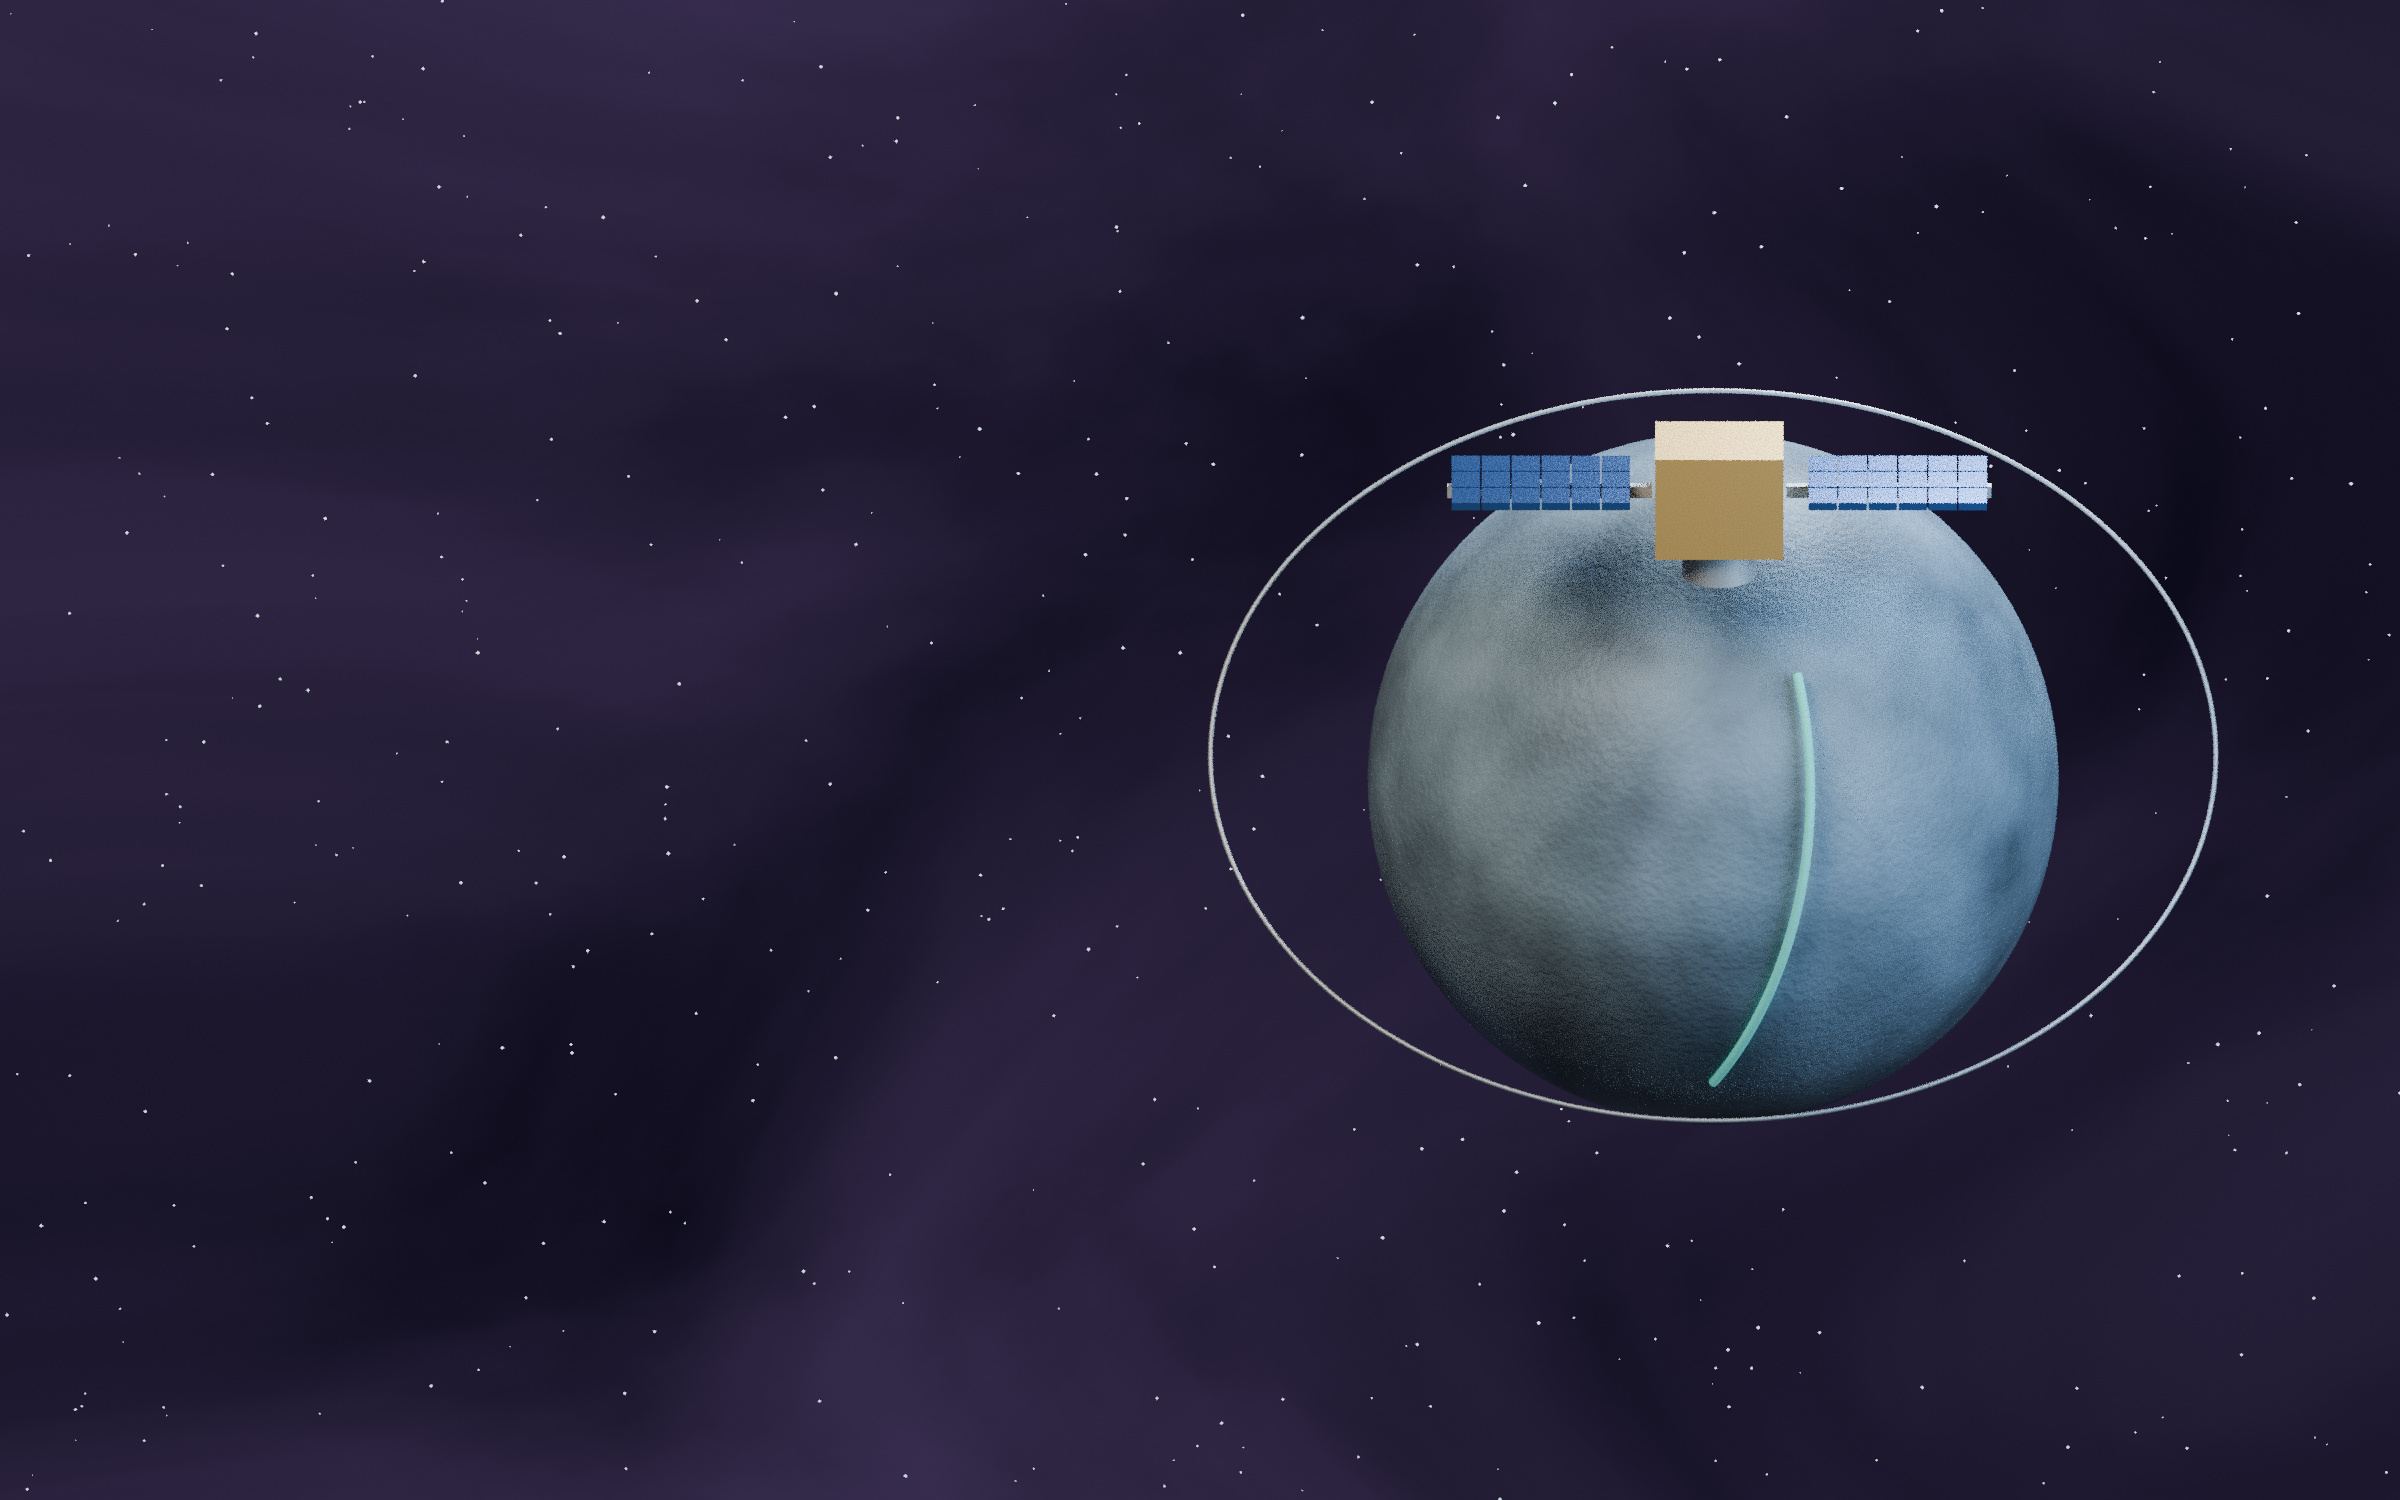
\includegraphics[width=20cm,height=12.5cm]{Scena/copertina.jpg}};}{}
\node[anchor=north west,inner sep=0] at([xshift=1.05cm,yshift=-1.10cm]current page.north west){\color{Mint}\bfseries\fontsize{23}{28}\selectfont ARGENTA};
\node[anchor=north west,inner sep=0] at([xshift=1.07cm,yshift=-2.16cm]current page.north west){\color{white}\fontsize{9}{12}\selectfont MODULO M15 · SCIENZE DELLA TERRA};
\draw[Mint,line width=1.5pt]([xshift=1.07cm,yshift=-2.78cm]current page.north west)--([xshift=2.6cm,yshift=-2.78cm]current page.north west);
\node[anchor=north west,inner sep=0] at([xshift=1.05cm,yshift=-3.35cm]current page.north west){\begin{minipage}{9.2cm}\raggedright\color{white}\bfseries\fontsize{28.5}{34.5}\selectfont Riproducibilità e\\progetto di analisi\end{minipage}};
\node[anchor=north west,inner sep=0] at([xshift=1.07cm,yshift=-7.88cm]current page.north west){\begin{minipage}{8.9cm}\raggedright\color{Lilac}\fontsize{12.2}{17}\selectfont Dalla misura al risultato verificabile\end{minipage}};
\node[anchor=north west,inner sep=0] at([xshift=1.07cm,yshift=-8.70cm]current page.north west){\begin{minipage}{8.9cm}\raggedright\color{white!75}\fontsize{10.3}{14.5}\selectfont Tracciabilità, tolleranze e scelte analitiche\end{minipage}};
\node[anchor=north west,inner sep=0] at([xshift=1.07cm,yshift=-10.52cm]current page.north west){\color{white}\fontsize{10.5}{14}\selectfont GeoStat Lab · corso di Marzio De Corato};
\node[anchor=north west,inner sep=0] at([xshift=1.07cm,yshift=-11.17cm]current page.north west){\color{Mint}\fontsize{8.8}{11}\selectfont\href{https://creativecommons.org/licenses/by-nc-sa/4.0/}{Impaginazione da Tessera · CC BY-NC-SA 4.0}};
\end{tikzpicture}\end{frame}
\begin{frame}[plain]\hypertarget{slide2}{}
\bookmark[level=1,page=2]{Indice della presentazione}
\begin{tikzpicture}[remember picture,overlay]
\PilotChrome{Indice della presentazione}{PERCORSO}{2}{I titoli dell’indice aprono i capitoli. Il nome del capitolo in alto riporta a questa pagina.}
\node[anchor=north west,inner sep=0] at([xshift=.96cm,yshift=-2.12cm]current page.north west){\Colonna{9.40cm}{\PLabel{Capitoli}
{\fontsize{10.7}{13.5}\selectfont\hyperlink{slide4}{Dati e dipendenze dell’analisi\hfill 4}\par}\vspace{.16cm}
{\fontsize{10.7}{13.5}\selectfont\hyperlink{slide12}{Identità e confronto numerico\hfill 12}\par}\vspace{.16cm}
{\fontsize{10.7}{13.5}\selectfont\hyperlink{slide24}{Funzioni e contratti di validità\hfill 24}\par}\vspace{.16cm}
{\fontsize{10.7}{13.5}\selectfont\hyperlink{slide35}{Casualità e ambiente di esecuzione\hfill 35}\par}\vspace{.16cm}
{\fontsize{10.7}{13.5}\selectfont\hyperlink{slide44}{Parametri, versioni e provenienza\hfill 44}\par}\vspace{.16cm}
}};
\node[anchor=north west,inner sep=0] at([xshift=10.85cm,yshift=-2.12cm]current page.north west){\Colonna{8.16cm}{\PLabel{Percorso di lettura}
\PBody{Riprendiamo i 24 provini del corso. Una tabella contiene masse, volumi e stazioni. Per rifare la sintesi servono anche regole di filtro, unità, codice e ambiente.}
\PInfo{Le pagine Scenario A e Confronto riprendono gli esperimenti nel browser. I valori di partenza del simulatore possono differire dal caso guida.}
\href{https://marzione00.github.io/Lab_Geo/\#modulo-M15}{\color{Classical}\bfseries Apri gli esperimenti di Argenta}}};
\end{tikzpicture}\end{frame}

\begin{frame}[plain]\hypertarget{slide3}{}
\bookmark[level=1,page=3]{Quali informazioni permettono di ricostruire la media delle densità di una stazione?}
\begin{tikzpicture}[remember picture,overlay]
\PilotChrome{{\fontsize{15.3}{19}\selectfont Quali informazioni permettono di ricostruire la media delle densità di una stazione?}}{IL CASO GUIDA}{3}{Un risultato ricostruibile conserva il legame fra dati, codice, parametri e ambiente.}
\node[anchor=north west,inner sep=0] at([xshift=.96cm,yshift=-2.12cm]current page.north west){\Colonna{9.40cm}{{\centering\resizebox{.97\linewidth}{!}{\begin{tikzpicture}[x=1cm,y=1cm]

\node[pFlow,text width=2.3cm] (m) at (1.5,3.6){Massa\\107,2 g};
\node[pFlow,text width=2.3cm] (v) at (1.5,1.4){Volume\\40 cm$^3$};
\node[pFlow,text width=2.25cm] (d) at (5.25,2.5){Densità C01\\2,68 g/cm$^3$};
\draw[pEdge] (m.east)--(d.west);\draw[pEdge](v.east)--(d.west);
\node[pFlow,text width=2.85cm] (s) at(5.25,.15){Media di A1\\2,685 g/cm$^3$};
\draw[pEdge](d)--(s);\node[pNote,anchor=east,text width=2.5cm] at(3.5,.15){altri tre\\provini di A1};
\draw[pEdge](3.5,.15)--(s);

\end{tikzpicture}
}\par}
}};
\node[anchor=north west,inner sep=0] at([xshift=10.85cm,yshift=-2.12cm]current page.north west){\Colonna{8.16cm}{\PLabel{Il caso}
\PBody{Riprendiamo i 24 provini del corso. Una tabella contiene masse, volumi e stazioni. Per rifare la sintesi servono anche regole di filtro, unità, codice e ambiente.}
\PInfo{Costruiremo una catena verificabile dalla riga C01 alla media della stazione A1. Ogni passaggio lascia un risultato confrontabile con un riferimento.}
}};
\end{tikzpicture}\end{frame}

\begin{frame}[plain]\hypertarget{slide4}{}
\bookmark[level=0,page=4]{Dati e dipendenze dell’analisi}
\bookmark[level=1,page=4]{Quali file servono per ricostruire una densità?}
\begin{tikzpicture}[remember picture,overlay]
\PilotChrome{Quali file servono per ricostruire una densità?}{DATI E DIPENDENZE DELL’ANALISI}{4}{Ogni risultato deve poter risalire agli input e alla trasformazione che lo ha prodotto.}
\node[anchor=north west,inner sep=0] at([xshift=.96cm,yshift=-2.12cm]current page.north west){\Colonna{9.40cm}{\PLabel{Domanda}
\PBody{Un archivio conserva le densità ma perde la tabella delle masse e dei volumi. Quale parte del risultato è ancora verificabile?}
\vspace{.35cm}\PLabel{Interpretazione}
\PBody{Una tabella finale permette di controllare una media. Per verificare le densità individuali occorrono le misure, le unità e la regola di trasformazione.}
}};
\node[anchor=north west,inner sep=0] at([xshift=10.85cm,yshift=-2.12cm]current page.north west){\Colonna{8.16cm}{\begin{tcolorbox}[enhanced,arc=1.7mm,boxrule=.6pt,colback=white,colframe=Classical!60!Navy,colbacktitle=Navy,coltitle=white,fonttitle=\bfseries\small,title={R · calcolo riproducibile},left=1.7mm,right=1.3mm,top=1.1mm,bottom=1.1mm,before skip=1mm,after skip=1.0mm]\lstinputlisting[style=GeoR,language=R]{Codice/capitolo-01.R}\end{tcolorbox}
\PLabel{Risultato in R}
\begin{tcolorbox}[colback=GeoTint,colframe=Rule,boxrule=.5pt,arc=1.4mm,left=2mm,right=1mm,top=1mm,bottom=1mm]{\fontsize{9}{12}\selectfont\ttfamily \mbox{id\ \ rho}\\\mbox{1\ C01\ 2.68}\\\mbox{2\ C02\ 2.71}\\\mbox{3\ C03\ 2.65}}\end{tcolorbox}}};
\end{tikzpicture}\end{frame}

\begin{frame}[plain]\hypertarget{slide5}{}
\bookmark[level=1,page=5]{Un risultato conserva la propria storia}
\begin{tikzpicture}[remember picture,overlay]
\PilotChrome{Un risultato conserva la propria storia}{DATI E DIPENDENZE DELL’ANALISI}{5}{La riproduzione del calcolo richiede una storia verificabile dei dati e delle scelte.}
\node[anchor=north west,inner sep=0] at([xshift=.96cm,yshift=-2.12cm]current page.north west){\Colonna{9.40cm}{{\centering\resizebox{.97\linewidth}{!}{\begin{tikzpicture}[x=1cm,y=-.87cm,every node/.style={font=\fontsize{12.2}{15}\selectfont,text=Ink},arr/.style={-{Stealth[length=2mm]},line width=.8pt,draw=Classical}]\path[use as bounding box] (0,0) rectangle (7.45,6.2);
\draw[draw=Classical,fill=Classical!8,rounded corners=2pt,line width=.7pt] (0.5,0.4) rectangle (6.9,1.5499999999999998);
\node[anchor=center,text=Ink,font=\fontsize{11.5}{15}\selectfont,text width=6cm,align=center] at (3.7,0.975) {Dati e protocollo di misura};
\draw[arr,draw=Classical] (3.7,1.7000000000000002)--(3.7,2.08);
\draw[draw=Quantum,fill=Quantum!8,rounded corners=2pt,line width=.7pt] (0.5,2.25) rectangle (6.9,3.4);
\node[anchor=center,text=Ink,font=\fontsize{11.5}{15}\selectfont,text width=6cm,align=center] at (3.7,2.825) {Trasformazioni e controlli};
\draw[arr,draw=Classical] (3.7,3.55)--(3.7,3.9299999999999997);
\draw[draw=Classical,fill=Classical!8,rounded corners=2pt,line width=.7pt] (0.5,4.1000000000000005) rectangle (6.9,5.25);
\node[anchor=center,text=Ink,font=\fontsize{11.5}{15}\selectfont,text width=6cm,align=center] at (3.7,4.675000000000001) {Risultato con provenienza};

\end{tikzpicture}}\par}
}};
\node[anchor=north west,inner sep=0] at([xshift=10.85cm,yshift=-2.12cm]current page.north west){\Colonna{8.16cm}{\PBody{Una tabella conclusiva acquista significato quando è possibile ricostruire i dati dai quali deriva, le trasformazioni applicate e le decisioni che ne hanno delimitato il contenuto. Il capitolo riprende ventiquattro provini distribuiti in sei stazioni e sviluppa una procedura per calcolare densità e medie di stazione. La ripetibilità del calcolo viene verificata separatamente dalla validità dell’interpretazione geologica, che dipende dal disegno di campionamento, dalla misura del volume e dalla rappresentatività delle stazioni.}
}};
\end{tikzpicture}\end{frame}

\begin{frame}[plain]\hypertarget{slide6}{}
\bookmark[level=1,page=6]{Separazione fra sorgenti e prodotti derivati}
\begin{tikzpicture}[remember picture,overlay]
\PilotChrome{Separazione fra sorgenti e prodotti derivati}{DATI E DIPENDENZE DELL’ANALISI}{6}{Ogni prodotto derivato deve poter essere ricostruito senza sovrascrivere l’input.}
\node[anchor=north west,inner sep=0] at([xshift=.96cm,yshift=-2.12cm]current page.north west){\Colonna{9.40cm}{{\centering\resizebox{.97\linewidth}{!}{\begin{tikzpicture}[x=1cm,y=-.87cm,every node/.style={font=\fontsize{12.2}{15}\selectfont,text=Ink},arr/.style={-{Stealth[length=2mm]},line width=.8pt,draw=Classical}]\path[use as bounding box] (0,0) rectangle (7.45,6.2);
\draw[draw=Classical,fill=Classical!8,rounded corners=2pt,line width=.7pt] (0.4,2.1) rectangle (2.6,3.6);
\node[anchor=center,text=Ink,font=\fontsize{12.2}{15}\selectfont,text width=1.9cm,align=center] at (1.5,2.85) {dati/};
\draw[arr,draw=Classical] (2.8,2.85)--(4.1,1.3);
\draw[arr,draw=Classical] (2.8,2.85)--(4.1,4.5);
\draw[draw=Quantum,fill=Quantum!8,rounded corners=2pt,line width=.7pt] (4.3,0.6) rectangle (7,2);
\node[anchor=center,text=Ink,font=\fontsize{12.2}{15}\selectfont,text width=2.4cm,align=center] at (5.65,1.3) {tabelle/};
\draw[draw=Classical,fill=Classical!8,rounded corners=2pt,line width=.7pt] (4.3,3.8) rectangle (7,5.2);
\node[anchor=center,text=Ink,font=\fontsize{12.2}{15}\selectfont,text width=2.4cm,align=center] at (5.65,4.5) {figure/};
\node[anchor=center,text=Ink,font=\fontsize{11}{15}\selectfont,text width=6.7cm,align=center] at (3.7,5.9) {Gli script dichiarano le dipendenze.};

\end{tikzpicture}}\par}
}};
\node[anchor=north west,inner sep=0] at([xshift=10.85cm,yshift=-2.12cm]current page.north west){\Colonna{8.16cm}{\PBody{I dati ricevuti vengono conservati in una cartella dedicata, mentre tabelle derivate, figure e registri di esecuzione sono scritti in destinazioni distinte. Questa organizzazione consente di ricostruire le trasformazioni e di confrontare una nuova elaborazione con la precedente. Una correzione del dato sorgente deve produrre una versione riconoscibile e una motivazione, affinché la differenza fra misura originaria e dato corretto rimanga documentata. La struttura delle cartelle esprime dunque una relazione di dipendenza fra oggetti scientifici.}
}};
\end{tikzpicture}\end{frame}

\begin{frame}[plain]\hypertarget{slide7}{}
\bookmark[level=1,page=7]{Il dizionario collega colonne e misure}
\begin{tikzpicture}[remember picture,overlay]
\PilotChrome{Il dizionario collega colonne e misure}{DATI E DIPENDENZE DELL’ANALISI}{7}{Il controllo dello schema deve essere accompagnato dalla verifica del significato delle variabili.}
\node[anchor=north west,inner sep=0] at([xshift=.96cm,yshift=-2.12cm]current page.north west){\Colonna{9.40cm}{\PLabel{Metodo}
\PBody{Il nome di una variabile permette di individuarla nel codice, mentre la sua interpretazione richiede unità, supporto della misura, metodo e convenzioni per i valori mancanti. Nel caso didattico, massa\_g e volume\_cm3 consentono una densità in grammi per centimetro cubo; l’identificativo distingue i provini e la stazione conserva il livello geografico del campionamento. Un controllo automatico può verificare la presenza delle colonne e l’unicità degli identificativi, mentre la pertinenza delle definizioni richiede conoscenza del protocollo.}
}};
\node[anchor=north west,inner sep=0] at([xshift=10.85cm,yshift=-2.12cm]current page.north west){\Colonna{8.16cm}{\PLabel{Formalismo}
\par\smallskip{\centering\adjustbox{max width=.98\linewidth}{$\displaystyle \rho_i=\frac{m_i}{V_i},\qquad [\rho]=\mathrm{g\,cm^{-3}}$}\par\smallskip}
\PLabel{Interpretazione}
\PBody{Per il provino i, $m_i$ è la massa in g, $V_i$ il volume in cm³ e $\rho_i$ la densità. Il dizionario associa a ogni colonna un significato, un’unità e un ruolo. Per gli identificativi si conserva il formato testuale; per le categorie si registrano i livelli ammessi; per le misure si dichiarano precisione, intervallo plausibile e codici di assenza.}
}};
\end{tikzpicture}\end{frame}

\begin{frame}[plain]\hypertarget{slide8}{}
\bookmark[level=1,page=8]{Radice del progetto e percorsi relativi}
\begin{tikzpicture}[remember picture,overlay]
\PilotChrome{Radice del progetto e percorsi relativi}{DATI E DIPENDENZE DELL’ANALISI}{8}{La cartella di avvio fa parte delle istruzioni necessarie a riprodurre un’analisi.}
\node[anchor=north west,inner sep=0] at([xshift=.96cm,yshift=-2.12cm]current page.north west){\Colonna{9.40cm}{\begin{tcolorbox}[enhanced,arc=1.7mm,boxrule=.6pt,colback=white,colframe=Classical!60!Navy,colbacktitle=Navy,coltitle=white,fonttitle=\bfseries\small,title={R · procedura},left=1.7mm,right=1.3mm,top=1.1mm,bottom=1.1mm,before skip=1mm,after skip=1.0mm]\lstinputlisting[style=GeoR,language=R]{Codice/lettura-06.R}\end{tcolorbox}
}};
\node[anchor=north west,inner sep=0] at([xshift=10.85cm,yshift=-2.12cm]current page.north west){\Colonna{8.16cm}{\PBody{Un percorso relativo viene interpretato rispetto alla cartella corrente, che può variare fra terminale, ambiente di sviluppo e documento eseguibile. La procedura del corso assume come radice la cartella contenente dati, R e sorgenti, dalla quale si avviano gli script. file.path compone i segmenti senza incorporare il percorso personale del docente. La verifica iniziale dell’esistenza del file permette di distinguere un errore di avvio da un problema di lettura o di contenuto della tabella.}
}};
\end{tikzpicture}\end{frame}

\begin{frame}[plain]\hypertarget{slide9}{}
\bookmark[level=1,page=9]{Un dizionario è un controllo sui dati in ingresso}
\begin{tikzpicture}[remember picture,overlay]
\PilotChrome{Un dizionario è un controllo sui dati in ingresso}{DATI E DIPENDENZE DELL’ANALISI}{9}{Unità, ruolo e tipo consentono di distinguere un codice di stazione da una quantità fisica.}
\node[anchor=north west,inner sep=0] at([xshift=.96cm,yshift=-2.12cm]current page.north west){\Colonna{9.40cm}{\PLabel{Risultati del calcolo in R}
{\fontsize{10.2}{12.8}\selectfont\begin{tabular}{@{}>{\raggedright\arraybackslash}p{0.31\linewidth}@{\hspace{.13cm}}>{\raggedright\arraybackslash}p{0.29\linewidth}@{\hspace{.13cm}}>{\raggedright\arraybackslash}p{0.32\linewidth}@{}}\toprule variabile & unita & ruolo\\[2.3pt]
\midrule 
id & identificativo & campione\\[2.3pt]
stazione & categoria & gruppo\\[2.3pt]
massa\_g & g & massa\\[2.3pt]
volume\_cm3 & cm3 & volume\\[2.3pt]
\bottomrule\end{tabular}\par}
}};
\node[anchor=north west,inner sep=0] at([xshift=10.85cm,yshift=-2.12cm]current page.north west){\Colonna{8.16cm}{\PBody{Quale informazione manca se si conserva soltanto il nome della colonna?}
\vspace{.4cm}\PInfo{Unità, ruolo e tipo consentono di distinguere un codice di stazione da una quantità fisica. Il dizionario è parte dell’input con cui si interpreta il CSV.}
}};
\node[anchor=north east,inner sep=0] at([xshift=17.1cm,yshift=-12.04cm]current page.north west){\fontsize{7.7}{9}\selectfont \href{https://github.com/marzione00/Lab_Geo/blob/649f7cc577b96bd1044d81e78a2f530813e4f96b/materiali/laboratori/M15/M15_N02.R}{\color{Classical}\bfseries Script R · M15\_N02}};
\end{tikzpicture}\end{frame}

\begin{frame}[plain]\hypertarget{slide10}{}
\bookmark[level=1,page=10]{Dipendenze fra dati e risultati}
\begin{tikzpicture}[remember picture,overlay]
\PilotChrome{Dipendenze fra dati e risultati}{DATI E DIPENDENZE DELL’ANALISI}{10}{Seguire l’effetto di una modifica al dato di ingresso.}
\node[anchor=north west,inner sep=0] at([xshift=.96cm,yshift=-2.12cm]current page.north west){\Colonna{9.40cm}{{\centering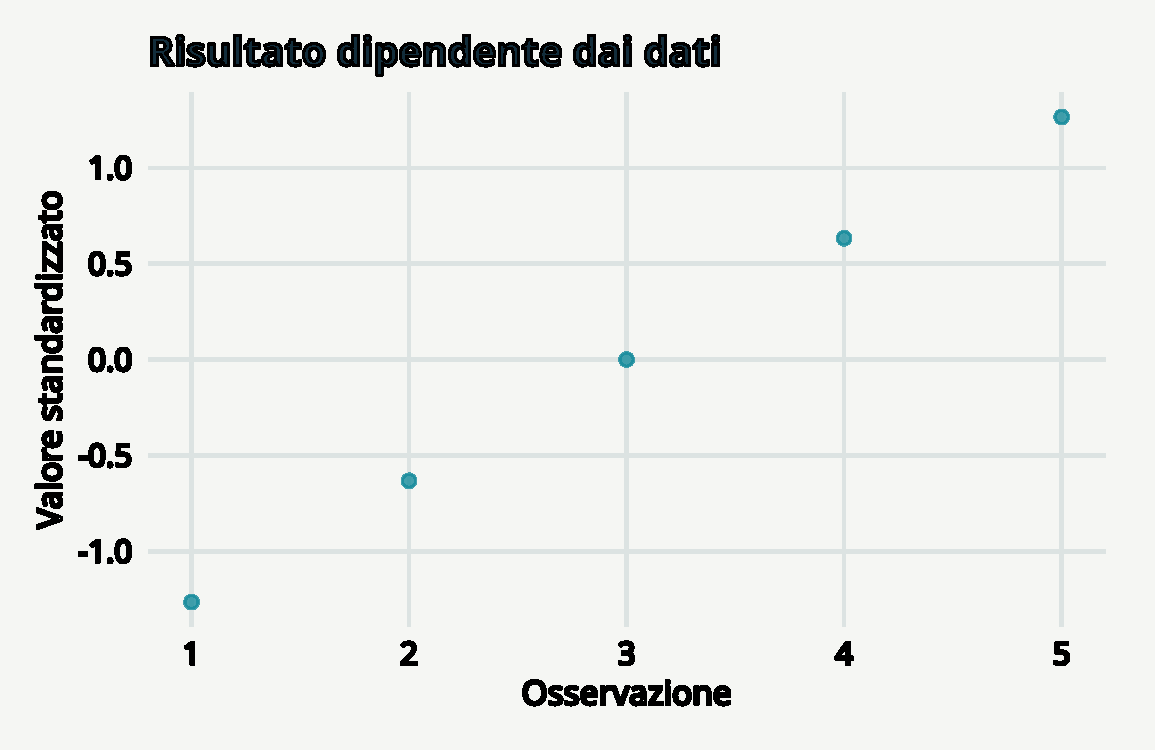
\includegraphics[width=\linewidth,height=6.0cm,keepaspectratio]{Esperimenti/m15-dipendenze-A.pdf}\par}
\PSmall{Ultima misura: 12. Seme: 17.}
}};
\node[anchor=north west,inner sep=0] at([xshift=10.85cm,yshift=-2.12cm]current page.north west){\Colonna{8.16cm}{\PLabel{Scenario A · simulazione}
\PBody{Un risultato analitico dipende dai dati e dalle trasformazioni che lo precedono. L’esperimento standardizza un breve vettore, sottraendone la media e dividendolo per la deviazione standard campionaria. Quando il controllo modifica l’ultima misura, cambiano entrambe le quantità di riferimento e vengono quindi ricalcolati anche i valori standardizzati delle osservazioni rimaste numericamente invariate.}
\par\smallskip{\centering\adjustbox{max width=.98\linewidth}{$\displaystyle D\longrightarrow f(D)\longrightarrow g(f(D))$}\par\smallskip}
\PSmall{D rappresenta il dato di ingresso; f è una prima trasformazione e g una trasformazione successiva. Nel caso concreto, media e deviazione standard dipendono dal vettore completo e determinano tutti i valori standardizzati.}
}};
\node[anchor=north east,inner sep=0] at([xshift=17.1cm,yshift=-12.04cm]current page.north west){\fontsize{7.7}{9}\selectfont \href{https://marzione00.github.io/Lab_Geo/\#laboratorio/m15-dipendenze}{\color{Classical}\bfseries Apri il laboratorio · m15-dipendenze}};
\end{tikzpicture}\end{frame}

\begin{frame}[plain]\hypertarget{slide11}{}
\bookmark[level=1,page=11]{Confronto | Dipendenze fra dati e risultati}
\begin{tikzpicture}[remember picture,overlay]
\PilotChrome{Confronto | Dipendenze fra dati e risultati}{DATI E DIPENDENZE DELL’ANALISI}{11}{Il grafo delle dipendenze rende verificabile la provenienza di ogni risultato.}
\node[anchor=north west,inner sep=0] at([xshift=.96cm,yshift=-2.12cm]current page.north west){\Colonna{9.40cm}{{\centering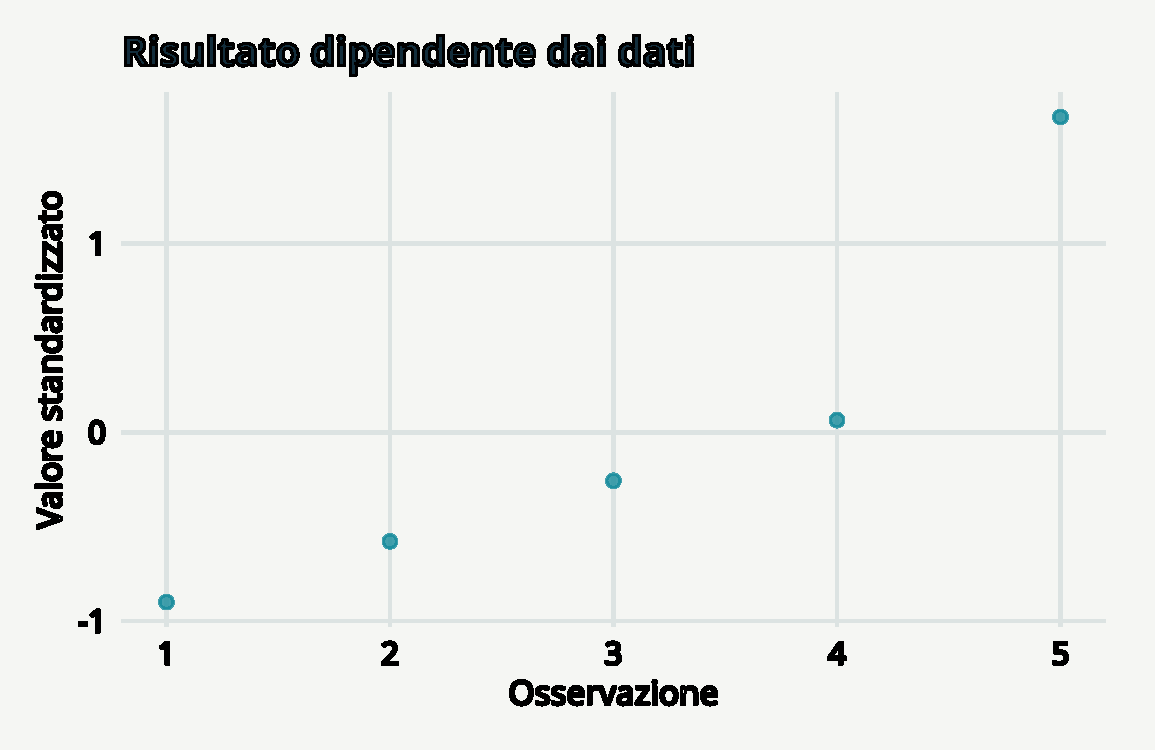
\includegraphics[width=\linewidth,height=5.6cm,keepaspectratio]{Esperimenti/m15-dipendenze-B.pdf}\par}
\PSmall{Ultima misura: 12 $\to$ 20. Tutti gli altri parametri e il seme sono fissi.}
}};
\node[anchor=north west,inner sep=0] at([xshift=10.85cm,yshift=-2.12cm]current page.north west){\Colonna{8.16cm}{\PLabel{Confronto fra gli scenari}
{\fontsize{10.2}{12.8}\selectfont\begin{tabular}{@{}>{\raggedright\arraybackslash}p{0.48\linewidth}@{\hspace{.13cm}}>{\raggedright\arraybackslash}p{0.224\linewidth}@{\hspace{.13cm}}>{\raggedright\arraybackslash}p{0.224\linewidth}@{}}\toprule Grandezza & A & B\\[2.3pt]
\midrule 
Media di ingresso & 8 & 9,6\\[2.3pt]
SD di ingresso & 3,16 & 6,23\\[2.3pt]
Media standardizzata & 0 & 6,94e-17\\[2.3pt]
Somma quadratica standardizzata & 4 & 4\\[2.3pt]
\bottomrule\end{tabular}\par}
\vspace{.25cm}\PBody{La media cambia insieme alla misura d’ingresso. La somma degli scarti centrati rimane vicina a zero, come richiede l’identità matematica.}
}};
\node[anchor=north east,inner sep=0] at([xshift=17.1cm,yshift=-12.04cm]current page.north west){\fontsize{7.7}{9}\selectfont \href{https://marzione00.github.io/Lab_Geo/\#laboratorio/m15-dipendenze}{\color{Classical}\bfseries Apri il laboratorio · m15-dipendenze}};
\end{tikzpicture}\end{frame}

\begin{frame}[plain]\hypertarget{slide12}{}
\bookmark[level=0,page=12]{Identità e confronto numerico}
\bookmark[level=1,page=12]{Un file può cambiare lasciando uguali i valori}
\begin{tikzpicture}[remember picture,overlay]
\PilotChrome{Un file può cambiare lasciando uguali i valori}{IDENTITÀ E CONFRONTO NUMERICO}{12}{Per verificare un archivio confronta i byte; per confrontare un calcolo dichiara tipo e tolleranza.}
\node[anchor=north west,inner sep=0] at([xshift=.96cm,yshift=-2.12cm]current page.north west){\Colonna{9.40cm}{\PLabel{Domanda}
\PBody{Un programma scrive 2,50 con due decimali, un altro scrive 2,5. Confrontiamo prima il testo, poi il valore numerico.}
\vspace{.35cm}\PLabel{Interpretazione}
\PBody{Due rappresentazioni diverse sono interpretabili come lo stesso numero. La domanda da porre determina il controllo da usare.}
}};
\node[anchor=north west,inner sep=0] at([xshift=10.85cm,yshift=-2.12cm]current page.north west){\Colonna{8.16cm}{\begin{tcolorbox}[enhanced,arc=1.7mm,boxrule=.6pt,colback=white,colframe=Classical!60!Navy,colbacktitle=Navy,coltitle=white,fonttitle=\bfseries\small,title={R · calcolo riproducibile},left=1.7mm,right=1.3mm,top=1.1mm,bottom=1.1mm,before skip=1mm,after skip=1.0mm]\lstinputlisting[style=GeoR,language=R]{Codice/capitolo-02.R}\end{tcolorbox}
\PLabel{Risultato in R}
\begin{tcolorbox}[colback=GeoTint,colframe=Rule,boxrule=.5pt,arc=1.4mm,left=2mm,right=1mm,top=1mm,bottom=1mm]{\fontsize{9}{12}\selectfont\ttfamily \mbox{testo\ valore\ }\\\mbox{\ FALSE\ \ \ TRUE}}\end{tcolorbox}}};
\end{tikzpicture}\end{frame}

\begin{frame}[plain]\hypertarget{slide13}{}
\bookmark[level=1,page=13]{Impronta dei byte ed equivalenza dei valori}
\begin{tikzpicture}[remember picture,overlay]
\PilotChrome{Impronta dei byte ed equivalenza dei valori}{IDENTITÀ E CONFRONTO NUMERICO}{13}{L’integrità del file e l’equivalenza scientifica del contenuto richiedono controlli distinti.}
\node[anchor=north west,inner sep=0] at([xshift=.96cm,yshift=-2.12cm]current page.north west){\Colonna{9.40cm}{{\centering\resizebox{.97\linewidth}{!}{\begin{tikzpicture}[x=1cm,y=-.87cm,every node/.style={font=\fontsize{12.2}{15}\selectfont,text=Ink},arr/.style={-{Stealth[length=2mm]},line width=.8pt,draw=Classical}]\path[use as bounding box] (0,0) rectangle (7.45,6.2);
\draw[draw=Classical,fill=Classical!8,rounded corners=2pt,line width=.7pt] (0.4,0.6) rectangle (3.4,2.1);
\node[anchor=center,text=Ink,font=\fontsize{16}{15}\selectfont,text width=2.6cm,align=center] at (1.9,1.35) {A,1};
\draw[draw=Quantum,fill=Quantum!8,rounded corners=2pt,line width=.7pt] (4,0.6) rectangle (7,2.1);
\node[anchor=center,text=Ink,font=\fontsize{16}{15}\selectfont,text width=2.6cm,align=center] at (5.5,1.35) {A,1.0};
\draw[arr,draw=Classical] (1.9,2.3)--(1.9,3.2);
\draw[arr,draw=Quantum] (5.5,2.3)--(5.5,3.2);
\node[anchor=center,text=Ink,font=\fontsize{12.2}{15}\selectfont,text width=2.8cm,align=center] at (1.9,3.8) {Byte differenti};
\node[anchor=center,text=Ink,font=\fontsize{12.2}{15}\selectfont,text width=2.8cm,align=center] at (5.5,3.8) {Valore uguale};
\node[anchor=center,text=Ink,font=\fontsize{11.5}{15}\selectfont,text width=6.7cm,align=center] at (3.7,5.3) {Due criteri di confronto rispondono a domande diverse.};

\end{tikzpicture}}\par}
}};
\node[anchor=north west,inner sep=0] at([xshift=10.85cm,yshift=-2.12cm]current page.north west){\Colonna{8.16cm}{\PBody{Un’impronta permette di confrontare un file con un riferimento prestabilito. Una differenza rileva una modifica della rappresentazione, che può riguardare anche soltanto un separatore o il numero di cifre stampate. Due CSV contenenti rispettivamente 1 e 1.0 possono quindi produrre impronte differenti e restituire lo stesso valore numerico dopo la lettura. Il manifest della consegna utilizza SHA-256; il laboratorio presenta anche MD5 come esempio di checksum, senza attribuirgli una funzione di sicurezza crittografica.}
}};
\end{tikzpicture}\end{frame}

\begin{frame}[plain]\hypertarget{slide14}{}
\bookmark[level=1,page=14]{Tolleranza assoluta e tolleranza relativa}
\begin{tikzpicture}[remember picture,overlay]
\PilotChrome{Tolleranza assoluta e tolleranza relativa}{IDENTITÀ E CONFRONTO NUMERICO}{14}{La tolleranza numerica deve essere definita rispetto all’operazione e alla scala dei valori.}
\node[anchor=north west,inner sep=0] at([xshift=.96cm,yshift=-2.12cm]current page.north west){\Colonna{9.40cm}{\PLabel{Metodo}
\PBody{Il confronto fra quantità numeriche richiede una soglia coerente con la loro scala e con l’errore computazionale atteso. Una componente assoluta protegge il confronto vicino allo zero, mentre una componente relativa cresce con il valore di riferimento. Le tolleranze di calcolo devono essere distinte dall’incertezza di misura: scegliere una soglia piccola verifica l’implementazione, senza rendere più preciso lo strumento. Nell’esempio si controlla la densità dopo esportazione e lettura, mantenendo invariati identificativi e ordine dei provini.}
}};
\node[anchor=north west,inner sep=0] at([xshift=10.85cm,yshift=-2.12cm]current page.north west){\Colonna{8.16cm}{\PLabel{Formalismo}
\par\smallskip{\centering\adjustbox{max width=.98\linewidth}{$\displaystyle |x-y|\leq\varepsilon_{\rm abs}+\varepsilon_{\rm rel}|x|$}\par\smallskip}
\PLabel{Interpretazione}
\PBody{$\varepsilon_{\rm abs}$ è la tolleranza assoluta, nelle unità di x; $\varepsilon_{\rm rel}$ è adimensionale. La regola assume x come riferimento; usare max(|x|, |y|) la rende simmetrica. Il codice di esportazione implementa esplicitamente la disuguaglianza. all.equal applica proprie convenzioni e restituisce TRUE oppure una descrizione; per un esito logico si usa isTRUE(all.equal(...)).}
}};
\end{tikzpicture}\end{frame}

\begin{frame}[plain]\hypertarget{slide15}{}
\bookmark[level=1,page=15]{Esportazione e rilettura come prova integrata}
\begin{tikzpicture}[remember picture,overlay]
\PilotChrome{Esportazione e rilettura come prova integrata}{IDENTITÀ E CONFRONTO NUMERICO}{15}{Una prova di esportazione verifica insieme contenuto, identità delle righe e convenzioni di lettura.}
\node[anchor=north west,inner sep=0] at([xshift=.96cm,yshift=-2.12cm]current page.north west){\Colonna{9.40cm}{\begin{tcolorbox}[enhanced,arc=1.7mm,boxrule=.6pt,colback=white,colframe=Classical!60!Navy,colbacktitle=Navy,coltitle=white,fonttitle=\bfseries\small,title={R · procedura},left=1.7mm,right=1.3mm,top=1.1mm,bottom=1.1mm,before skip=1mm,after skip=1.0mm]\lstinputlisting[style=GeoR,language=R]{Codice/lettura-09.R}\end{tcolorbox}
}};
\node[anchor=north west,inner sep=0] at([xshift=10.85cm,yshift=-2.12cm]current page.north west){\Colonna{8.16cm}{\PBody{La prova di andata e ritorno coinvolge scrittura, formato del file, interpretazione delle colonne e recupero dei valori. Il controllo degli identificativi impedisce che una tabella numericamente plausibile nasconda un riordinamento o la perdita di righe. Per le densità si applica una tolleranza esplicita, mentre i codici di assenza vengono dichiarati in entrambe le direzioni. Il file temporaneo consente di eseguire la verifica senza introdurre un nuovo input nella cartella dei dati sorgente.}
}};
\end{tikzpicture}\end{frame}

\begin{frame}[plain]\hypertarget{slide16}{}
\bookmark[level=1,page=16]{Arrotondamento e perdita di informazione}
\begin{tikzpicture}[remember picture,overlay]
\PilotChrome{Arrotondamento e perdita di informazione}{IDENTITÀ E CONFRONTO NUMERICO}{16}{La precisione di stampa deve essere scelta dopo le trasformazioni che utilizzano i valori.}
\node[anchor=north west,inner sep=0] at([xshift=.96cm,yshift=-2.12cm]current page.north west){\Colonna{9.40cm}{{\centering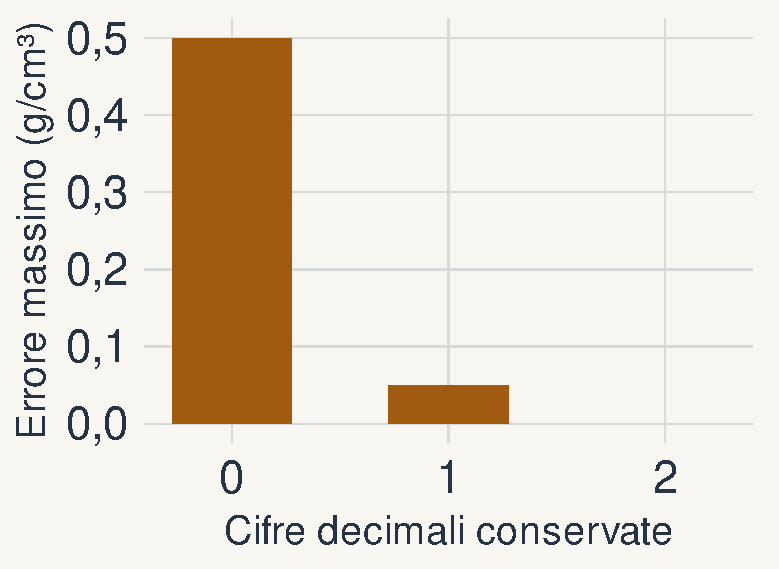
\includegraphics[width=\linewidth,height=6.15cm,keepaspectratio]{Figure/F03.pdf}\par}
\PSmall{Errore assoluto massimo rispetto alle densità calcolate. Il valore a due decimali è nullo entro la precisione macchina.}
}};
\node[anchor=north west,inner sep=0] at([xshift=10.85cm,yshift=-2.12cm]current page.north west){\Colonna{8.16cm}{\PBody{Arrotondare i risultati prima di completarli introduce un errore che può propagarsi nelle operazioni successive. La figura confronta l’errore massimo sulle densità conservando zero, una o due cifre decimali. Nel dataset didattico le densità sono state costruite con due decimali, per cui questa precisione recupera i valori entro l’approssimazione numerica. Il caso distingue la formattazione destinata alla lettura dalla precisione conservata nel calcolo: una tabella può mostrare poche cifre lasciando disponibili valori più precisi nel file di lavoro.}
}};
\end{tikzpicture}\end{frame}

\begin{frame}[plain]\hypertarget{slide17}{}
\bookmark[level=1,page=17]{Zero, assenza e convenzione di scambio}
\begin{tikzpicture}[remember picture,overlay]
\PilotChrome{Zero, assenza e convenzione di scambio}{IDENTITÀ E CONFRONTO NUMERICO}{17}{Il trattamento dei mancanti è una decisione scientifica successiva al riconoscimento del loro codice.}
\node[anchor=north west,inner sep=0] at([xshift=.96cm,yshift=-2.12cm]current page.north west){\Colonna{9.40cm}{{\centering\resizebox{.97\linewidth}{!}{\begin{tikzpicture}[x=1cm,y=-.87cm,every node/.style={font=\fontsize{12.2}{15}\selectfont,text=Ink},arr/.style={-{Stealth[length=2mm]},line width=.8pt,draw=Classical}]\path[use as bounding box] (0,0) rectangle (7.45,6.2);
\draw[draw=Classical,fill=Classical!8,rounded corners=2pt,line width=.7pt] (0.6,0.8) rectangle (2.7,2.6);
\node[anchor=center,text=Ink,font=\fontsize{24}{15}\selectfont] at (1.65,1.7) {0};
\draw[draw=Quantum,fill=Quantum!8,rounded corners=2pt,line width=.7pt] (4.7,0.8) rectangle (6.8,2.6);
\node[anchor=center,text=Ink,font=\fontsize{22}{15}\selectfont] at (5.75,1.7) {NA};
\node[anchor=center,text=Ink,font=\fontsize{12.2}{15}\selectfont,text width=2.8cm,align=center] at (1.65,3.6) {Valore misurato};
\node[anchor=center,text=Ink,font=\fontsize{12.2}{15}\selectfont,text width=2.8cm,align=center] at (5.75,3.6) {Valore assente};
\node[anchor=center,text=Ink,font=\fontsize{11.5}{15}\selectfont,text width=6.5cm,align=center] at (3.7,5.3) {Il codice di assenza si conserva nello scambio.};

\end{tikzpicture}}\par}
}};
\node[anchor=north west,inner sep=0] at([xshift=10.85cm,yshift=-2.12cm]current page.north west){\Colonna{8.16cm}{\PBody{Uno zero rappresenta un valore, mentre NA indica che il valore non è disponibile secondo la convenzione adottata. Un campo vuoto può assumere significati diversi nei programmi che leggono il file, per cui il formato di scambio deve specificare il codice utilizzato. La scelta di escludere i mancanti da una sintesi modifica l’insieme delle osservazioni considerate e richiede una motivazione rispetto al processo che ha prodotto l’assenza. La conservazione del codice durante l’esportazione precede tale decisione analitica.}
}};
\end{tikzpicture}\end{frame}

\begin{frame}[plain]\hypertarget{slide18}{}
\bookmark[level=1,page=18]{Il viaggio di andata e ritorno coinvolge anche gli ID}
\begin{tikzpicture}[remember picture,overlay]
\PilotChrome{Il viaggio di andata e ritorno coinvolge anche gli ID}{IDENTITÀ E CONFRONTO NUMERICO}{18}{Nel caso di riferimento le 24 righe ritornano con identificativi coerenti e scarto nullo sulla massa.}
\node[anchor=north west,inner sep=0] at([xshift=.96cm,yshift=-2.12cm]current page.north west){\Colonna{9.40cm}{\PLabel{Risultati del calcolo in R}
{\fontsize{10.2}{12.8}\selectfont\begin{tabular}{@{}>{\raggedright\arraybackslash}p{0.52\linewidth}@{\hspace{.13cm}}>{\raggedright\arraybackslash}p{0.39\linewidth}@{}}\toprule Grandezza & Valore\\[2.3pt]
\midrule 
Numero & 24\\[2.3pt]
ID & sì\\[2.3pt]
Scarto massa & 0\\[2.3pt]
\bottomrule\end{tabular}\par}
}};
\node[anchor=north west,inner sep=0] at([xshift=10.85cm,yshift=-2.12cm]current page.north west){\Colonna{8.16cm}{\PBody{Che cosa verifica una rilettura del file dopo la scrittura?}
\vspace{.4cm}\PInfo{Nel caso di riferimento le 24 righe ritornano con identificativi coerenti e scarto nullo sulla massa. Controllare solo il numero di righe avrebbe lasciato aperto il rischio di un riordino.}
}};
\node[anchor=north east,inner sep=0] at([xshift=17.1cm,yshift=-12.04cm]current page.north west){\fontsize{7.7}{9}\selectfont \href{https://github.com/marzione00/Lab_Geo/blob/649f7cc577b96bd1044d81e78a2f530813e4f96b/materiali/laboratori/M15/M15_N04.R}{\color{Classical}\bfseries Script R · M15\_N04}};
\end{tikzpicture}\end{frame}

\begin{frame}[plain]\hypertarget{slide19}{}
\bookmark[level=1,page=19]{Zero e campo vuoto restano distinguibili}
\begin{tikzpicture}[remember picture,overlay]
\PilotChrome{Zero e campo vuoto restano distinguibili}{IDENTITÀ E CONFRONTO NUMERICO}{19}{Lo zero conserva un significato numerico.}
\node[anchor=north west,inner sep=0] at([xshift=.96cm,yshift=-2.12cm]current page.north west){\Colonna{9.40cm}{\PLabel{Risultati del calcolo in R}
{\fontsize{10.2}{12.8}\selectfont\begin{tabular}{@{}>{\raggedright\arraybackslash}p{0.44\linewidth}@{\hspace{.13cm}}>{\raggedright\arraybackslash}p{0.48\linewidth}@{}}\toprule id & valore\\[2.3pt]
\midrule 
1 & 0\\[2.3pt]
2 & NA\\[2.3pt]
3 & 2\\[2.3pt]
\bottomrule\end{tabular}\par}
}};
\node[anchor=north west,inner sep=0] at([xshift=10.85cm,yshift=-2.12cm]current page.north west){\Colonna{8.16cm}{\PBody{Quali valori devono tornare leggendo una colonna che contiene una misura nulla e una mancante?}
\vspace{.4cm}\PInfo{Lo zero conserva un significato numerico. Il valore mancante rimane escluso o propagato secondo la regola statistica dichiarata.}
}};
\node[anchor=north east,inner sep=0] at([xshift=17.1cm,yshift=-12.04cm]current page.north west){\fontsize{7.7}{9}\selectfont \href{https://github.com/marzione00/Lab_Geo/blob/649f7cc577b96bd1044d81e78a2f530813e4f96b/materiali/laboratori/M15/M15_N09.R}{\color{Classical}\bfseries Script R · M15\_N09}};
\end{tikzpicture}\end{frame}

\begin{frame}[plain]\hypertarget{slide20}{}
\bookmark[level=1,page=20]{Identità e confronto numerico}
\begin{tikzpicture}[remember picture,overlay]
\PilotChrome{Identità e confronto numerico}{IDENTITÀ E CONFRONTO NUMERICO}{20}{Scegliere una tolleranza coerente con la scala del problema.}
\node[anchor=north west,inner sep=0] at([xshift=.96cm,yshift=-2.12cm]current page.north west){\Colonna{9.40cm}{{\centering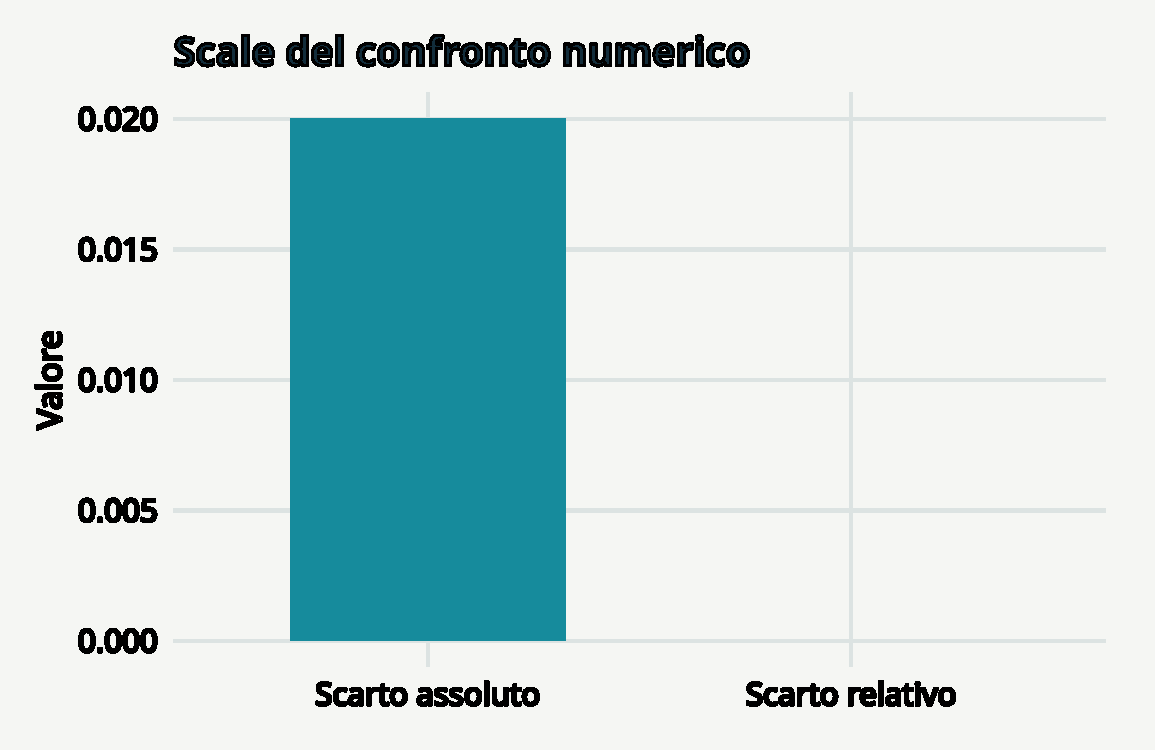
\includegraphics[width=\linewidth,height=6.0cm,keepaspectratio]{Esperimenti/m15-tolleranze-A.pdf}\par}
\PSmall{Ordine di grandezza: 10\textasciicircum{}k: 6. Seme: 17.}
}};
\node[anchor=north west,inner sep=0] at([xshift=10.85cm,yshift=-2.12cm]current page.north west){\Colonna{8.16cm}{\PLabel{Scenario A · simulazione}
\PBody{Un confronto numerico deve distinguere la grandezza dello scarto dalla scala dei valori confrontati. Il programma costruisce due numeri che differiscono per una perturbazione relativa controllabile; un secondo parametro ne modifica l’ordine di grandezza. Lo scarto assoluto e quello relativo vengono riportati separatamente, insieme all’esito di un criterio che combina entrambe le tolleranze.}
\par\smallskip{\centering\adjustbox{max width=.98\linewidth}{$\displaystyle |a-b|\le\epsilon_{abs}+\epsilon_{rel}\max(|a|,|b|)$}\par\smallskip}
\PSmall{a e b sono i numeri confrontati; $\varepsilon_{\mathrm{abs}}$ è la tolleranza assoluta e $\varepsilon_{\mathrm{rel}}$ quella relativa. Lo scarto relativo mostrato divide $|a-b|$ per il massimo fra i loro valori assoluti.}
}};
\node[anchor=north east,inner sep=0] at([xshift=17.1cm,yshift=-12.04cm]current page.north west){\fontsize{7.7}{9}\selectfont \href{https://marzione00.github.io/Lab_Geo/\#laboratorio/m15-tolleranze}{\color{Classical}\bfseries Apri il laboratorio · m15-tolleranze}};
\end{tikzpicture}\end{frame}

\begin{frame}[plain]\hypertarget{slide21}{}
\bookmark[level=1,page=21]{Confronto | Identità e confronto numerico}
\begin{tikzpicture}[remember picture,overlay]
\PilotChrome{Confronto | Identità e confronto numerico}{IDENTITÀ E CONFRONTO NUMERICO}{21}{Una soglia numerica deve essere dichiarata insieme al criterio che la utilizza.}
\node[anchor=north west,inner sep=0] at([xshift=.96cm,yshift=-2.12cm]current page.north west){\Colonna{9.40cm}{{\centering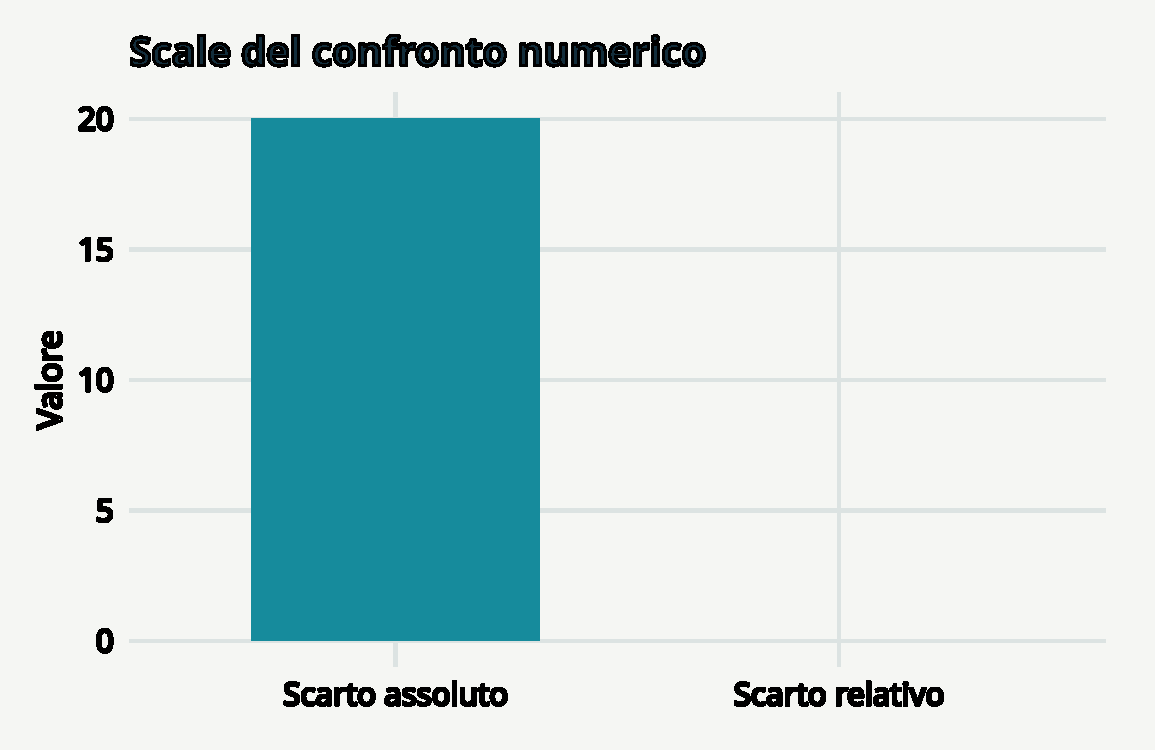
\includegraphics[width=\linewidth,height=5.6cm,keepaspectratio]{Esperimenti/m15-tolleranze-B.pdf}\par}
\PSmall{Ordine di grandezza: 10\textasciicircum{}k: 6 $\to$ 9. Tutti gli altri parametri e il seme sono fissi.}
}};
\node[anchor=north west,inner sep=0] at([xshift=10.85cm,yshift=-2.12cm]current page.north west){\Colonna{8.16cm}{\PLabel{Confronto fra gli scenari}
{\fontsize{10.2}{12.8}\selectfont\begin{tabular}{@{}>{\raggedright\arraybackslash}p{0.48\linewidth}@{\hspace{.13cm}}>{\raggedright\arraybackslash}p{0.224\linewidth}@{\hspace{.13cm}}>{\raggedright\arraybackslash}p{0.224\linewidth}@{}}\toprule Grandezza & A & B\\[2.3pt]
\midrule 
Scarto assoluto & 0,02 & 20\\[2.3pt]
Scarto relativo & 2,00e-08 & 2,00e-08\\[2.3pt]
Esito con εabs=$10^{-6}$, εrel=$10^{-8}$ & no & no\\[2.3pt]
\bottomrule\end{tabular}\par}
\vspace{.25cm}\PBody{Lo scarto assoluto passa da 0,02 a 20. Lo scarto relativo resta uguale perché la perturbazione cresce insieme alla scala del riferimento.}
}};
\node[anchor=north east,inner sep=0] at([xshift=17.1cm,yshift=-12.04cm]current page.north west){\fontsize{7.7}{9}\selectfont \href{https://marzione00.github.io/Lab_Geo/\#laboratorio/m15-tolleranze}{\color{Classical}\bfseries Apri il laboratorio · m15-tolleranze}};
\end{tikzpicture}\end{frame}

\begin{frame}[plain]\hypertarget{slide22}{}
\bookmark[level=1,page=22]{Integrità dei file e identità dei dati}
\begin{tikzpicture}[remember picture,overlay]
\PilotChrome{Integrità dei file e identità dei dati}{IDENTITÀ E CONFRONTO NUMERICO}{22}{Confrontare contenuto numerico, rappresentazione testuale e impronta di un file.}
\node[anchor=north west,inner sep=0] at([xshift=.96cm,yshift=-2.12cm]current page.north west){\Colonna{9.40cm}{{\centering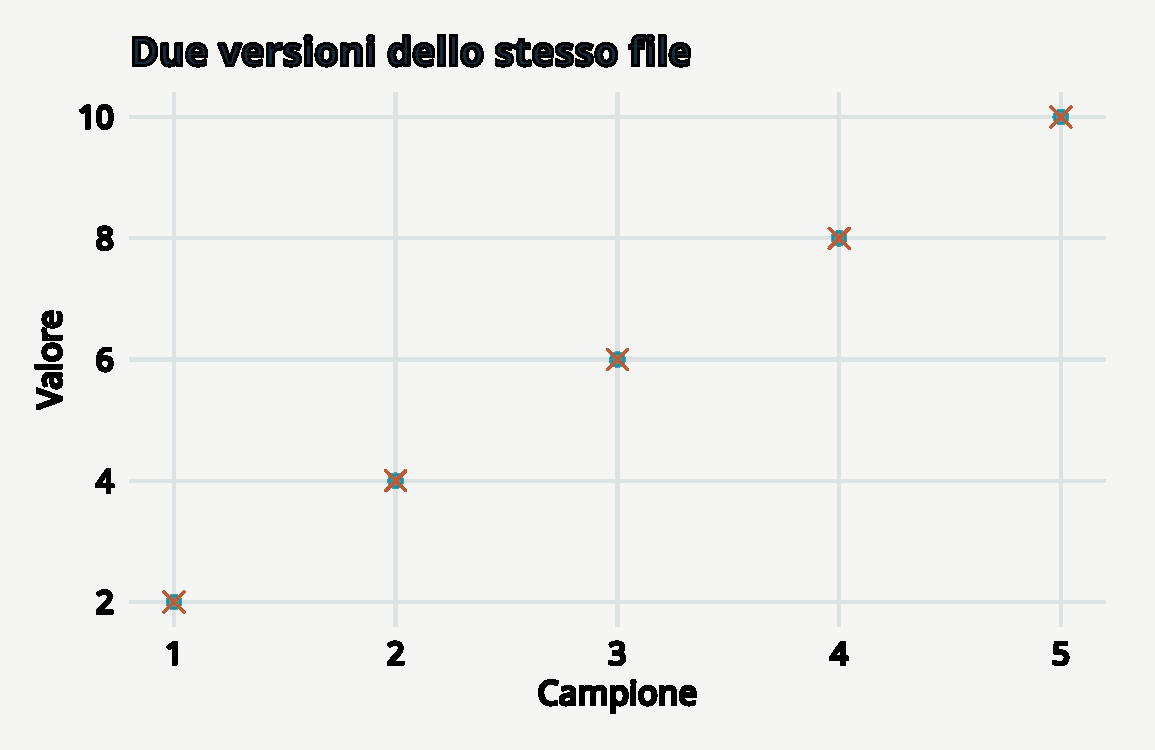
\includegraphics[width=\linewidth,height=6.0cm,keepaspectratio]{Esperimenti/m15-integrita-A.pdf}\par}
\PSmall{Variazione dell’ultima misura: 0. Seme: 17.}
}};
\node[anchor=north west,inner sep=0] at([xshift=10.85cm,yshift=-2.12cm]current page.north west){\Colonna{8.16cm}{\PLabel{Scenario A · simulazione}
\PBody{L’attività scrive due tabelle in file CSV temporanei, dopo avere applicato alla seconda una variazione controllata dell’ultima misura. Vengono quindi confrontati valori numerici, sequenze di byte e impronte MD5, rendendo esplicito il passaggio dalla tabella in memoria al contenuto persistente.}
\par\smallskip{\centering\adjustbox{max width=.98\linewidth}{$\displaystyle D_A=D_B\Longrightarrow h(D_A)=h(D_B)$}\par\smallskip}
\PSmall{$D_A$ e $D_B$ sono le sequenze di byte dei due file; $h$ è la funzione di impronta. L’implicazione scritta procede dall’identità dei file all’uguaglianza delle impronte.}
}};
\node[anchor=north east,inner sep=0] at([xshift=17.1cm,yshift=-12.04cm]current page.north west){\fontsize{7.7}{9}\selectfont \href{https://marzione00.github.io/Lab_Geo/\#laboratorio/m15-integrita}{\color{Classical}\bfseries Apri il laboratorio · m15-integrita}};
\end{tikzpicture}\end{frame}

\begin{frame}[plain]\hypertarget{slide23}{}
\bookmark[level=1,page=23]{Confronto | Integrità dei file e identità dei dati}
\begin{tikzpicture}[remember picture,overlay]
\PilotChrome{Confronto | Integrità dei file e identità dei dati}{IDENTITÀ E CONFRONTO NUMERICO}{23}{La ricostruzione conserva il file effettivamente analizzato e documenta quando il suo contenuto cambia.}
\node[anchor=north west,inner sep=0] at([xshift=.96cm,yshift=-2.12cm]current page.north west){\Colonna{9.40cm}{{\centering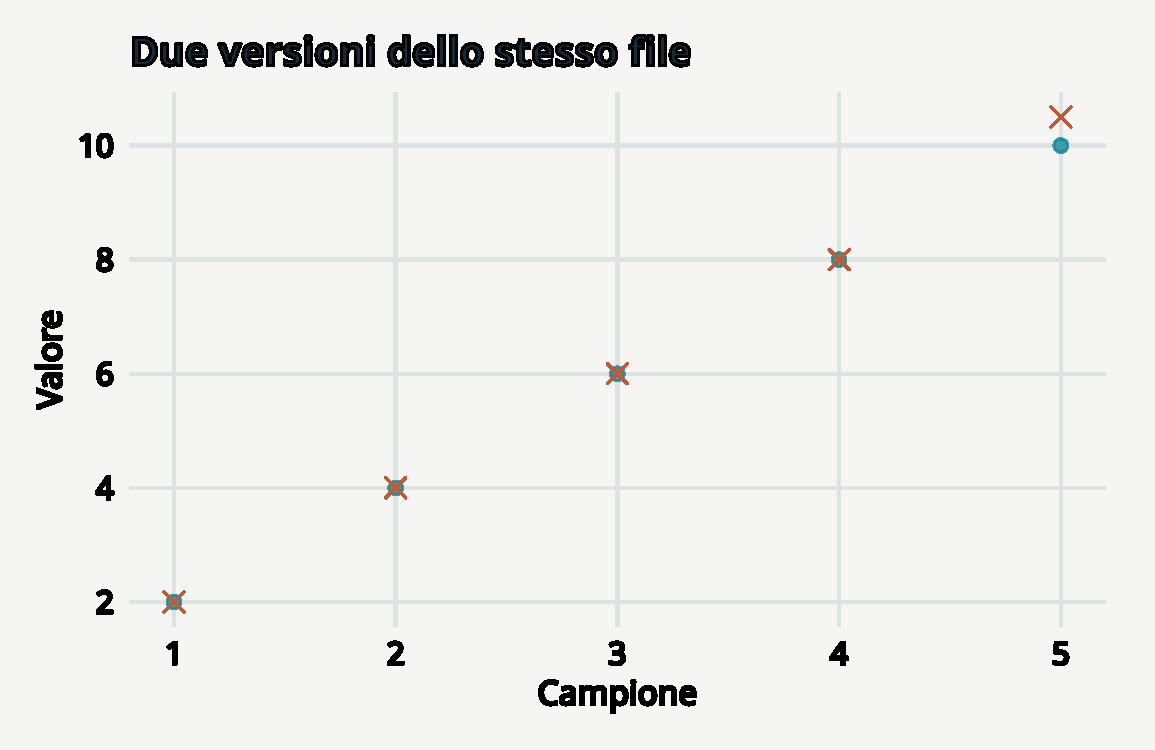
\includegraphics[width=\linewidth,height=5.6cm,keepaspectratio]{Esperimenti/m15-integrita-B.pdf}\par}
\PSmall{Variazione dell’ultima misura: 0 $\to$ 0,5. Tutti gli altri parametri e il seme sono fissi.}
}};
\node[anchor=north west,inner sep=0] at([xshift=10.85cm,yshift=-2.12cm]current page.north west){\Colonna{8.16cm}{\PLabel{Confronto fra gli scenari}
{\fontsize{10.2}{12.8}\selectfont\begin{tabular}{@{}>{\raggedright\arraybackslash}p{0.48\linewidth}@{\hspace{.13cm}}>{\raggedright\arraybackslash}p{0.224\linewidth}@{\hspace{.13cm}}>{\raggedright\arraybackslash}p{0.224\linewidth}@{}}\toprule Grandezza & A & B\\[2.3pt]
\midrule 
Byte identici & sì & no\\[2.3pt]
Impronta A & eb826a… & eb826a…\\[2.3pt]
Impronta B & eb826a… & 406e5e…\\[2.3pt]
Scarto numerico massimo & 0 & 0,5\\[2.3pt]
\bottomrule\end{tabular}\par}
\vspace{.25cm}\PBody{Con una variazione di 0,5, la seconda impronta cambia e lo scarto numerico diventa osservabile. Le impronte sono usate qui per confrontare copie didattiche.}
}};
\node[anchor=north east,inner sep=0] at([xshift=17.1cm,yshift=-12.04cm]current page.north west){\fontsize{7.7}{9}\selectfont \href{https://marzione00.github.io/Lab_Geo/\#laboratorio/m15-integrita}{\color{Classical}\bfseries Apri il laboratorio · m15-integrita}};
\end{tikzpicture}\end{frame}

\begin{frame}[plain]\hypertarget{slide24}{}
\bookmark[level=0,page=24]{Funzioni e contratti di validità}
\bookmark[level=1,page=24]{Se il volume è zero, il calcolo deve fermarsi}
\begin{tikzpicture}[remember picture,overlay]
\PilotChrome{Se il volume è zero, il calcolo deve fermarsi}{FUNZIONI E CONTRATTI DI VALIDITÀ}{24}{Valida il dominio fisico oltre al tipo numerico.}
\node[anchor=north west,inner sep=0] at([xshift=.96cm,yshift=-2.12cm]current page.north west){\Colonna{9.40cm}{\PLabel{Domanda}
\PBody{Un errore di importazione trasforma un volume mancante in zero. Che cosa può verificare una funzione prima della divisione?}
\vspace{.35cm}\PLabel{Interpretazione}
\PBody{Una precondizione rende visibile il problema all’ingresso. Il controllo del caso valido protegge anche il comportamento atteso della funzione.}
}};
\node[anchor=north west,inner sep=0] at([xshift=10.85cm,yshift=-2.12cm]current page.north west){\Colonna{8.16cm}{\begin{tcolorbox}[enhanced,arc=1.7mm,boxrule=.6pt,colback=white,colframe=Classical!60!Navy,colbacktitle=Navy,coltitle=white,fonttitle=\bfseries\small,title={R · calcolo riproducibile},left=1.7mm,right=1.3mm,top=1.1mm,bottom=1.1mm,before skip=1mm,after skip=1.0mm]\lstinputlisting[style=GeoR,language=R]{Codice/capitolo-03.R}\end{tcolorbox}
\PLabel{Risultato in R}
\begin{tcolorbox}[colback=GeoTint,colframe=Rule,boxrule=.5pt,arc=1.4mm,left=2mm,right=1mm,top=1mm,bottom=1mm]{\fontsize{9}{12}\selectfont\ttfamily \mbox{valida\ rifiuta\_zero\ }\\\mbox{\ \ \ \ \ \ \ \ \ 2.5\ \ \ \ \ \ \ \ \ \ 1.0}}\end{tcolorbox}}};
\end{tikzpicture}\end{frame}

\begin{frame}[plain]\hypertarget{slide25}{}
\bookmark[level=1,page=25]{Una funzione dichiara il proprio dominio}
\begin{tikzpicture}[remember picture,overlay]
\PilotChrome{Una funzione dichiara il proprio dominio}{FUNZIONI E CONTRATTI DI VALIDITÀ}{25}{I controlli dell’input traducono in condizioni eseguibili il dominio dichiarato della funzione.}
\node[anchor=north west,inner sep=0] at([xshift=.96cm,yshift=-2.12cm]current page.north west){\Colonna{9.40cm}{\begin{tcolorbox}[enhanced,arc=1.7mm,boxrule=.6pt,colback=white,colframe=Classical!60!Navy,colbacktitle=Navy,coltitle=white,fonttitle=\bfseries\small,title={R · procedura},left=1.7mm,right=1.3mm,top=1.1mm,bottom=1.1mm,before skip=1mm,after skip=1.0mm]\lstinputlisting[style=GeoR,language=R]{Codice/lettura-12.R}\end{tcolorbox}
\par\smallskip{\centering\adjustbox{max width=.98\linewidth}{$\displaystyle f:\mathbb R_{>0}^2\to\mathbb R_{>0},\qquad f(m,V)=m/V$}\par\smallskip}
}};
\node[anchor=north west,inner sep=0] at([xshift=10.85cm,yshift=-2.12cm]current page.north west){\Colonna{8.16cm}{\PBody{La funzione di densità richiede masse e volumi numerici, finiti, positivi e della stessa lunghezza. Il controllo delle lunghezze evita il riciclo implicito dei vettori, che potrebbe associare masse e volumi in modo diverso da quello previsto. Un volume nullo viene intercettato prima della divisione e produce un errore riconoscibile. Il contratto descrive le condizioni necessarie al calcolo, mentre la plausibilità dei valori e la corrispondenza fra provino e misura richiedono ulteriori controlli del protocollo.}
}};
\end{tikzpicture}\end{frame}

\begin{frame}[plain]\hypertarget{slide26}{}
\bookmark[level=1,page=26]{Composizione delle trasformazioni}
\begin{tikzpicture}[remember picture,overlay]
\PilotChrome{Composizione delle trasformazioni}{FUNZIONI E CONTRATTI DI VALIDITÀ}{26}{La scomposizione espone gli oggetti intermedi sui quali verificare il procedimento.}
\node[anchor=north west,inner sep=0] at([xshift=.96cm,yshift=-2.12cm]current page.north west){\Colonna{9.40cm}{{\centering\resizebox{.97\linewidth}{!}{\begin{tikzpicture}[x=1cm,y=-.87cm,every node/.style={font=\fontsize{12.2}{15}\selectfont,text=Ink},arr/.style={-{Stealth[length=2mm]},line width=.8pt,draw=Classical}]\path[use as bounding box] (0,0) rectangle (7.45,6.2);
\draw[draw=Classical,fill=Classical!8,rounded corners=2pt,line width=.7pt] (0.5,0.4) rectangle (6.9,1.5499999999999998);
\node[anchor=center,text=Ink,font=\fontsize{11.5}{15}\selectfont,text width=6cm,align=center] at (3.7,0.975) {V: verifica del dominio};
\draw[arr,draw=Classical] (3.7,1.7000000000000002)--(3.7,2.08);
\draw[draw=Quantum,fill=Quantum!8,rounded corners=2pt,line width=.7pt] (0.5,2.25) rectangle (6.9,3.4);
\node[anchor=center,text=Ink,font=\fontsize{11.5}{15}\selectfont,text width=6cm,align=center] at (3.7,2.825) {T: densità di ogni provino};
\draw[arr,draw=Classical] (3.7,3.55)--(3.7,3.9299999999999997);
\draw[draw=Classical,fill=Classical!8,rounded corners=2pt,line width=.7pt] (0.5,4.1000000000000005) rectangle (6.9,5.25);
\node[anchor=center,text=Ink,font=\fontsize{11.5}{15}\selectfont,text width=6cm,align=center] at (3.7,4.675000000000001) {S: sintesi per stazione};

\end{tikzpicture}}\par}
\PSmall{D: tabella sorgente; Y: sintesi per stazione. La composizione si legge da destra a sinistra: prima V, poi T, infine S.}
}};
\node[anchor=north west,inner sep=0] at([xshift=10.85cm,yshift=-2.12cm]current page.north west){\Colonna{8.16cm}{\PBody{Una procedura può essere scomposta in lettura, validazione, trasformazione e sintesi. Ogni passaggio produce un oggetto il cui contenuto può essere controllato prima di procedere, riducendo la difficoltà di localizzare un errore. Nel caso della densità, la trasformazione aggiunge una colonna a una copia della tabella, mentre la sintesi raggruppa i provini per stazione. La funzione restituisce il risultato senza modificare l’input e senza dipendere da variabili nascoste nella sessione di lavoro.}
\par\smallskip{\centering\adjustbox{max width=.98\linewidth}{$\displaystyle Y=(S\circ T\circ V)(D)$}\par\smallskip}
}};
\end{tikzpicture}\end{frame}

\begin{frame}[plain]\hypertarget{slide27}{}
\bookmark[level=1,page=27]{Ripetibilità e idempotenza sono proprietà diverse}
\begin{tikzpicture}[remember picture,overlay]
\PilotChrome{Ripetibilità e idempotenza sono proprietà diverse}{FUNZIONI E CONTRATTI DI VALIDITÀ}{27}{La proprietà da verificare deve essere formulata prima di scrivere il confronto.}
\node[anchor=north west,inner sep=0] at([xshift=.96cm,yshift=-2.12cm]current page.north west){\Colonna{9.40cm}{\PLabel{Metodo}
\PBody{Una funzione deterministica restituisce lo stesso risultato quando riceve gli stessi input e opera nello stesso ambiente. L’idempotenza richiede invece che applicare nuovamente la funzione al suo risultato lasci quest’ultimo invariato. Il raddoppio di un numero è deterministico, pur modificando ancora il valore se viene ripetuto sull’uscita. La distinzione permette di formulare prove appropriate: il confronto fra due esecuzioni della procedura parte entrambe le volte dalla medesima tabella sorgente.}
}};
\node[anchor=north west,inner sep=0] at([xshift=10.85cm,yshift=-2.12cm]current page.north west){\Colonna{8.16cm}{\PLabel{Formalismo}
\par\smallskip{\centering\adjustbox{max width=.98\linewidth}{$\displaystyle y_1=f(D;\eta),\quad y_2=f(D;\eta)\Rightarrow y_1=y_2$}\par\smallskip}

\par\smallskip{\centering\adjustbox{max width=.98\linewidth}{$\displaystyle f(f(D))=f(D)\quad\text{per funzioni idempotenti}$}\par\smallskip}
\PLabel{Interpretazione}
\PBody{$\eta$ raccoglie ambiente e condizioni di esecuzione. Per f(x) = 2x, due chiamate con x = 3 restituiscono entrambe 6, mentre f(f(3)) vale 12. Un filtro che conserva soltanto volumi positivi è idempotente, purché l’uscita resti un input ammissibile.}
}};
\end{tikzpicture}\end{frame}

\begin{frame}[plain]\hypertarget{slide28}{}
\bookmark[level=1,page=28]{Esempi manuali, casi limite e invarianti}
\begin{tikzpicture}[remember picture,overlay]
\PilotChrome{Esempi manuali, casi limite e invarianti}{FUNZIONI E CONTRATTI DI VALIDITÀ}{28}{Le prove più utili confrontano l’implementazione con un riferimento indipendente o una proprietà sostanziale.}
\node[anchor=north west,inner sep=0] at([xshift=.96cm,yshift=-2.12cm]current page.north west){\Colonna{9.40cm}{{\centering\resizebox{.97\linewidth}{!}{\begin{tikzpicture}[x=1cm,y=-.87cm,every node/.style={font=\fontsize{12.2}{15}\selectfont,text=Ink},arr/.style={-{Stealth[length=2mm]},line width=.8pt,draw=Classical}]\path[use as bounding box] (0,0) rectangle (7.45,6.2);
\draw[draw=Classical,fill=Classical!8,rounded corners=2pt,line width=.7pt] (0.6,0.5) rectangle (6.8,1.7);
\node[anchor=center,text=Ink,font=\fontsize{12.2}{15}\selectfont,text width=5.9cm,align=center] at (3.7,1.1) {Valore noto: $10/4=2{,}5$};
\draw[draw=Quantum,fill=Quantum!8,rounded corners=2pt,line width=.7pt] (0.6,2.4) rectangle (6.8,3.6);
\node[anchor=center,text=Ink,font=\fontsize{12.2}{15}\selectfont,text width=5.9cm,align=center] at (3.7,3) {Caso limite: volume nullo};
\draw[draw=Measure,fill=Measure!8,rounded corners=2pt,line width=.7pt] (0.6,4.3) rectangle (6.8,5.5);
\node[anchor=center,text=Ink,font=\fontsize{12.2}{15}\selectfont,text width=5.9cm,align=center] at (3.7,4.9) {Invariante: stessi identificativi};

\end{tikzpicture}}\par}
}};
\node[anchor=north west,inner sep=0] at([xshift=10.85cm,yshift=-2.12cm]current page.north west){\Colonna{8.16cm}{\PBody{Un valore calcolabile a mano offre un riferimento indipendente per verificare la formula, mentre i casi limite mettono alla prova il dominio della funzione. Gli invarianti esprimono proprietà che devono restare vere durante una trasformazione, come la conservazione degli identificativi dopo l’aggiunta della densità. La riuscita di queste prove aumenta la fiducia nell’implementazione entro i casi esaminati; la copertura va estesa quando emergono nuovi errori o nuove condizioni d’uso, evitando confronti che ripetano semplicemente lo stesso codice da verificare.}
}};
\end{tikzpicture}\end{frame}

\begin{frame}[plain]\hypertarget{slide29}{}
\bookmark[level=1,page=29]{Densità dei provini e sintesi delle stazioni}
\begin{tikzpicture}[remember picture,overlay]
\PilotChrome{Densità dei provini e sintesi delle stazioni}{FUNZIONI E CONTRATTI DI VALIDITÀ}{29}{La sintesi conserva il livello geografico al quale appartengono le osservazioni.}
\node[anchor=north west,inner sep=0] at([xshift=.96cm,yshift=-2.12cm]current page.north west){\Colonna{9.40cm}{{\centering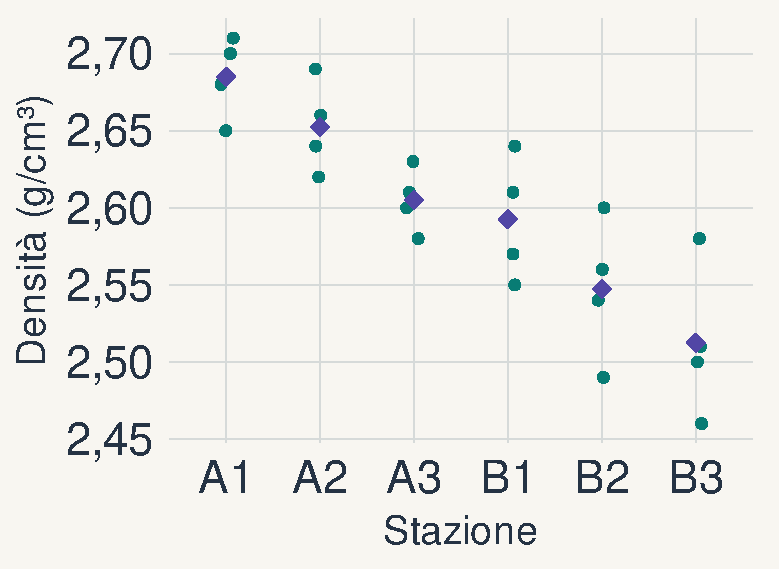
\includegraphics[width=\linewidth,height=6.15cm,keepaspectratio]{Figure/F01.pdf}\par}
\PSmall{$\rho_i$: densità del provino i; $n_s=4$: provini della stazione s. Verde: valori individuali; rombi viola: sei medie di stazione.}
}};
\node[anchor=north west,inner sep=0] at([xshift=10.85cm,yshift=-2.12cm]current page.north west){\Colonna{8.16cm}{\PBody{La figura conserva le ventiquattro osservazioni individuali e sovrappone le sei medie di stazione, rendendo visibili sia la variabilità interna sia le differenze fra gruppi. I punti sono leggermente separati in orizzontale per facilitarne la lettura, senza alterare i valori verticali. La sintesi costituisce l’uscita della procedura deterministica, mentre un’inferenza sulle differenze fra affioramenti richiederebbe di rispettare la struttura gerarchica del campionamento. La disponibilità di quattro provini per stazione non moltiplica automaticamente le repliche geografiche.}
\par\smallskip{\centering\adjustbox{max width=.98\linewidth}{$\displaystyle \overline\rho_s=\frac1{n_s}\sum_{i\in s}\rho_i$}\par\smallskip}
}};
\end{tikzpicture}\end{frame}

\begin{frame}[plain]\hypertarget{slide30}{}
\bookmark[level=1,page=30]{Una misura fisica richiede precondizioni verificabili}
\begin{tikzpicture}[remember picture,overlay]
\PilotChrome{Una misura fisica richiede precondizioni verificabili}{FUNZIONI E CONTRATTI DI VALIDITÀ}{30}{Il caso valido produce la densità attesa.}
\node[anchor=north west,inner sep=0] at([xshift=.96cm,yshift=-2.12cm]current page.north west){\Colonna{9.40cm}{\PLabel{Risultati del calcolo in R}
{\fontsize{10.2}{12.8}\selectfont\begin{tabular}{@{}>{\raggedright\arraybackslash}p{0.44\linewidth}@{\hspace{.13cm}}>{\raggedright\arraybackslash}p{0.48\linewidth}@{}}\toprule densita & Errore rilevato\\[2.3pt]
\midrule 
2,5 & sì\\[2.3pt]
2,5 & sì\\[2.3pt]
\bottomrule\end{tabular}\par}
}};
\node[anchor=north west,inner sep=0] at([xshift=10.85cm,yshift=-2.12cm]current page.north west){\Colonna{8.16cm}{\PBody{Che cosa succede a un provino con volume incompatibile con il calcolo?}
\vspace{.4cm}\PInfo{Il caso valido produce la densità attesa. Il controllo sul caso impossibile intercetta l’errore prima che il valore entri nella sintesi di stazione.}
}};
\node[anchor=north east,inner sep=0] at([xshift=17.1cm,yshift=-12.04cm]current page.north west){\fontsize{7.7}{9}\selectfont \href{https://github.com/marzione00/Lab_Geo/blob/649f7cc577b96bd1044d81e78a2f530813e4f96b/materiali/laboratori/M15/M15_N10.R}{\color{Classical}\bfseries Script R · M15\_N10}};
\end{tikzpicture}\end{frame}

\begin{frame}[plain]\hypertarget{slide31}{}
\bookmark[level=1,page=31]{Una trasformazione può preservare i dati in ingresso}
\begin{tikzpicture}[remember picture,overlay]
\PilotChrome{Una trasformazione può preservare i dati in ingresso}{FUNZIONI E CONTRATTI DI VALIDITÀ}{31}{Il confronto verifica sia la ripetibilità dell’output sia la conservazione dell’input.}
\node[anchor=north west,inner sep=0] at([xshift=.96cm,yshift=-2.12cm]current page.north west){\Colonna{9.40cm}{\PLabel{Risultati del calcolo in R}
{\fontsize{10.2}{12.8}\selectfont\begin{tabular}{@{}>{\raggedright\arraybackslash}p{0.52\linewidth}@{\hspace{.13cm}}>{\raggedright\arraybackslash}p{0.39\linewidth}@{}}\toprule Grandezza & Valore\\[2.3pt]
\midrule 
Input invariato & sì\\[2.3pt]
identico & sì\\[2.3pt]
\bottomrule\end{tabular}\par}
}};
\node[anchor=north west,inner sep=0] at([xshift=10.85cm,yshift=-2.12cm]current page.north west){\Colonna{8.16cm}{\PBody{Due chiamate alla funzione hanno modificato il campione di partenza?}
\vspace{.4cm}\PInfo{Il confronto verifica sia la ripetibilità dell’output sia la conservazione dell’input. Sono proprietà distinte e meritano controlli distinti.}
}};
\node[anchor=north east,inner sep=0] at([xshift=17.1cm,yshift=-12.04cm]current page.north west){\fontsize{7.7}{9}\selectfont \href{https://github.com/marzione00/Lab_Geo/blob/649f7cc577b96bd1044d81e78a2f530813e4f96b/materiali/laboratori/M15/M15_N11.R}{\color{Classical}\bfseries Script R · M15\_N11}};
\end{tikzpicture}\end{frame}

\begin{frame}[plain]\hypertarget{slide32}{}
\bookmark[level=1,page=32]{Un test piccolo rende leggibile il riferimento}
\begin{tikzpicture}[remember picture,overlay]
\PilotChrome{Un test piccolo rende leggibile il riferimento}{FUNZIONI E CONTRATTI DI VALIDITÀ}{32}{Prima si controlla un rapporto noto, poi si esaminano dominio e tolleranza.}
\node[anchor=north west,inner sep=0] at([xshift=.96cm,yshift=-2.12cm]current page.north west){\Colonna{9.40cm}{\PLabel{Risultati del calcolo in R}
{\fontsize{10.2}{12.8}\selectfont\begin{tabular}{@{}>{\raggedright\arraybackslash}p{0.44\linewidth}@{\hspace{.13cm}}>{\raggedright\arraybackslash}p{0.48\linewidth}@{}}\toprule test & passa\\[2.3pt]
\midrule 
densita nota & sì\\[2.3pt]
ricostruzione & sì\\[2.3pt]
\bottomrule\end{tabular}\par}
}};
\node[anchor=north west,inner sep=0] at([xshift=10.85cm,yshift=-2.12cm]current page.north west){\Colonna{8.16cm}{\PBody{Quali proprietà si possono verificare con un provino costruito a mano?}
\vspace{.4cm}\PInfo{Prima si controlla un rapporto noto, poi si esaminano dominio e tolleranza. Il test resta eseguibile anche quando il dataset principale cambia.}
}};
\node[anchor=north east,inner sep=0] at([xshift=17.1cm,yshift=-12.04cm]current page.north west){\fontsize{7.7}{9}\selectfont \href{https://github.com/marzione00/Lab_Geo/blob/649f7cc577b96bd1044d81e78a2f530813e4f96b/materiali/laboratori/M15/M15_N12.R}{\color{Classical}\bfseries Script R · M15\_N12}};
\end{tikzpicture}\end{frame}

\begin{frame}[plain]\hypertarget{slide33}{}
\bookmark[level=1,page=33]{Verificare una funzione prima dell’uso}
\begin{tikzpicture}[remember picture,overlay]
\PilotChrome{Verificare una funzione prima dell’uso}{FUNZIONI E CONTRATTI DI VALIDITÀ}{33}{Sottoporre una funzione a casi validi e invalidi.}
\node[anchor=north west,inner sep=0] at([xshift=.96cm,yshift=-2.12cm]current page.north west){\Colonna{9.40cm}{{\centering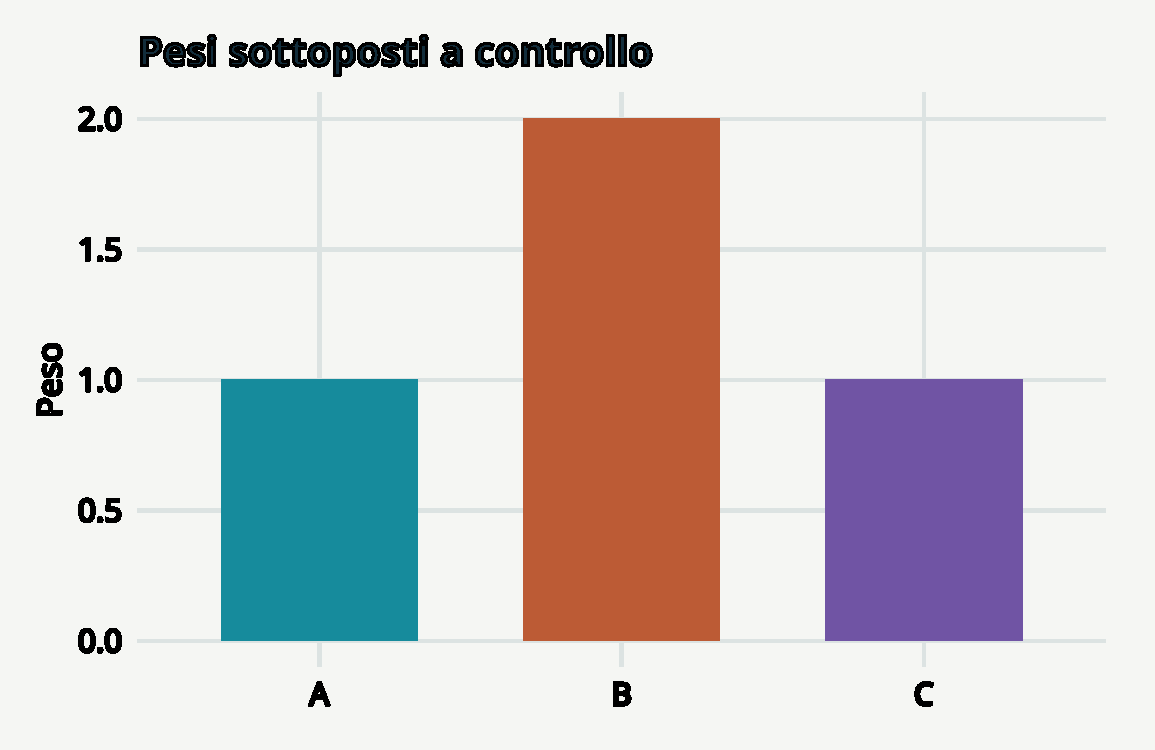
\includegraphics[width=\linewidth,height=6.0cm,keepaspectratio]{Esperimenti/m15-contratti-A.pdf}\par}
\PSmall{Caso di controllo: Pesi validi. Seme: 17.}
}};
\node[anchor=north west,inner sep=0] at([xshift=10.85cm,yshift=-2.12cm]current page.north west){\Colonna{8.16cm}{\PLabel{Scenario A · simulazione}
\PBody{Il contratto di una funzione specifica le condizioni nelle quali il risultato possiede il significato previsto. L’esperimento considera una media pesata con pesi finiti, non negativi e somma positiva. Le configurazioni disponibili permettono di confrontare un ingresso valido con pesi che violano una o più condizioni, mentre la carta rende visibile il vettore sottoposto a verifica.}
\par\smallskip{\centering\adjustbox{max width=.98\linewidth}{$\displaystyle \bar x_w=\frac{\sum_iw_ix_i}{\sum_iw_i},\quad w_i\ge0,\quad\sum_iw_i>0$}\par\smallskip}
\PSmall{$x_i$ è il valore dell’osservazione i e $w_i$ il peso assegnato. La media pesata divide la somma dei prodotti $w_i x_i$ per la somma dei pesi; il dominio qui dichiarato richiede $w_i$$\geq$0 e somma strettamente positiva.}
}};
\node[anchor=north east,inner sep=0] at([xshift=17.1cm,yshift=-12.04cm]current page.north west){\fontsize{7.7}{9}\selectfont \href{https://marzione00.github.io/Lab_Geo/\#laboratorio/m15-contratti}{\color{Classical}\bfseries Apri il laboratorio · m15-contratti}};
\end{tikzpicture}\end{frame}

\begin{frame}[plain]\hypertarget{slide34}{}
\bookmark[level=1,page=34]{Confronto | Verificare una funzione prima dell’uso}
\begin{tikzpicture}[remember picture,overlay]
\PilotChrome{Confronto | Verificare una funzione prima dell’uso}{FUNZIONI E CONTRATTI DI VALIDITÀ}{34}{I controlli esplicitano il dominio della funzione e distinguono errori d’ingresso da risultati ammessi.}
\node[anchor=north west,inner sep=0] at([xshift=.96cm,yshift=-2.12cm]current page.north west){\Colonna{9.40cm}{{\centering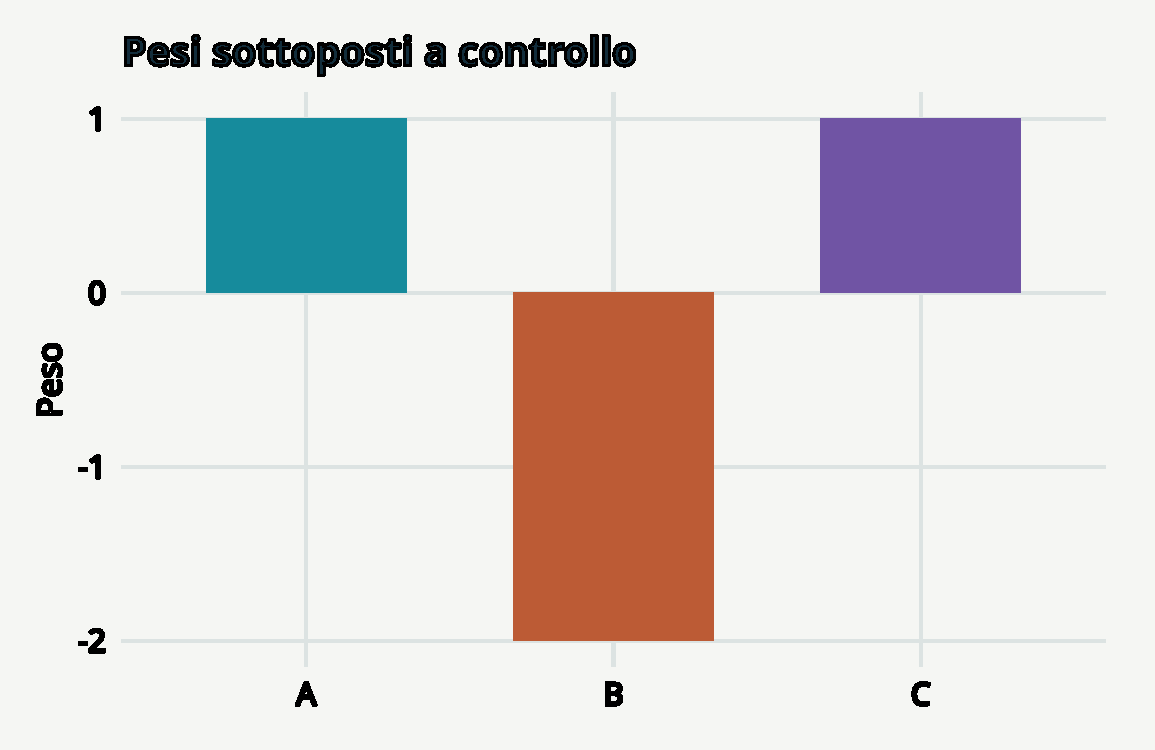
\includegraphics[width=\linewidth,height=5.6cm,keepaspectratio]{Esperimenti/m15-contratti-B.pdf}\par}
\PSmall{Caso di controllo: Pesi validi $\to$ Un peso negativo. Tutti gli altri parametri e il seme sono fissi.}
}};
\node[anchor=north west,inner sep=0] at([xshift=10.85cm,yshift=-2.12cm]current page.north west){\Colonna{8.16cm}{\PLabel{Confronto fra gli scenari}
{\fontsize{10.2}{12.8}\selectfont\begin{tabular}{@{}>{\raggedright\arraybackslash}p{0.48\linewidth}@{\hspace{.13cm}}>{\raggedright\arraybackslash}p{0.224\linewidth}@{\hspace{.13cm}}>{\raggedright\arraybackslash}p{0.224\linewidth}@{}}\toprule Grandezza & A & B\\[2.3pt]
\midrule 
Pesi non negativi & sì & no\\[2.3pt]
Somma positiva & sì & no\\[2.3pt]
Risultato & 5,25 & Input respinto dal contratto\\[2.3pt]
\bottomrule\end{tabular}\par}
\vspace{.25cm}\PBody{Un peso negativo fa fallire il controllo del dominio. Il rifiuto è l’esito previsto per un ingresso incompatibile con la media pesata definita.}
}};
\node[anchor=north east,inner sep=0] at([xshift=17.1cm,yshift=-12.04cm]current page.north west){\fontsize{7.7}{9}\selectfont \href{https://marzione00.github.io/Lab_Geo/\#laboratorio/m15-contratti}{\color{Classical}\bfseries Apri il laboratorio · m15-contratti}};
\end{tikzpicture}\end{frame}

\begin{frame}[plain]\hypertarget{slide35}{}
\bookmark[level=0,page=35]{Casualità e ambiente di esecuzione}
\bookmark[level=1,page=35]{Un piano di indici rende visibile il campionamento}
\begin{tikzpicture}[remember picture,overlay]
\PilotChrome{Un piano di indici rende visibile il campionamento}{CASUALITÀ E AMBIENTE DI ESECUZIONE}{35}{Documenta gli indici e la convenzione usata per interpretarli.}
\node[anchor=north west,inner sep=0] at([xshift=.96cm,yshift=-2.12cm]current page.north west){\Colonna{9.40cm}{\PLabel{Domanda}
\PBody{Tre valori sono ricampionati usando gli indici 2, 2, 1. Questo singolo piano può essere passato identico a R o Python.}
\vspace{.35cm}\PLabel{Interpretazione}
\PBody{Conservando gli indici si risale ai dati che hanno prodotto la media ricampionata. In Python la prima posizione ha indice zero e il piano va convertito.}
}};
\node[anchor=north west,inner sep=0] at([xshift=10.85cm,yshift=-2.12cm]current page.north west){\Colonna{8.16cm}{\begin{tcolorbox}[enhanced,arc=1.7mm,boxrule=.6pt,colback=white,colframe=Classical!60!Navy,colbacktitle=Navy,coltitle=white,fonttitle=\bfseries\small,title={R · calcolo riproducibile},left=1.7mm,right=1.3mm,top=1.1mm,bottom=1.1mm,before skip=1mm,after skip=1.0mm]\lstinputlisting[style=GeoR,language=R]{Codice/capitolo-04.R}\end{tcolorbox}
\PLabel{Risultato in R}
\begin{tcolorbox}[colback=GeoTint,colframe=Rule,boxrule=.5pt,arc=1.4mm,left=2mm,right=1mm,top=1mm,bottom=1mm]{\fontsize{9}{12}\selectfont\ttfamily \mbox{media\ }\\\mbox{\ 2.71\ \ 2.71\ \ 2.68\ \ 2.70}}\end{tcolorbox}}};
\end{tikzpicture}\end{frame}

\begin{frame}[plain]\hypertarget{slide36}{}
\bookmark[level=1,page=36]{Il seme identifica una sequenza in un ambiente}
\begin{tikzpicture}[remember picture,overlay]
\PilotChrome{Il seme identifica una sequenza in un ambiente}{CASUALITÀ E AMBIENTE DI ESECUZIONE}{36}{La sequenza dipende dall’intero procedimento di generazione.}
\node[anchor=north west,inner sep=0] at([xshift=.96cm,yshift=-2.12cm]current page.north west){\Colonna{9.40cm}{{\centering\resizebox{.97\linewidth}{!}{\begin{tikzpicture}[x=1cm,y=-.87cm,every node/.style={font=\fontsize{12.2}{15}\selectfont,text=Ink},arr/.style={-{Stealth[length=2mm]},line width=.8pt,draw=Classical}]\path[use as bounding box] (0,0) rectangle (7.45,6.2);
\draw[draw=Classical,fill=Classical!8,rounded corners=2pt,line width=.7pt] (0.5,0.4) rectangle (6.9,1.5499999999999998);
\node[anchor=center,text=Ink,font=\fontsize{11.5}{15}\selectfont,text width=6cm,align=center] at (3.7,0.975) {Seme e algoritmo dichiarati};
\draw[arr,draw=Classical] (3.7,1.7000000000000002)--(3.7,2.08);
\draw[draw=Quantum,fill=Quantum!8,rounded corners=2pt,line width=.7pt] (0.5,2.25) rectangle (6.9,3.4);
\node[anchor=center,text=Ink,font=\fontsize{11.5}{15}\selectfont,text width=6cm,align=center] at (3.7,2.825) {Stato e ordine delle chiamate};
\draw[arr,draw=Classical] (3.7,3.55)--(3.7,3.9299999999999997);
\draw[draw=Classical,fill=Classical!8,rounded corners=2pt,line width=.7pt] (0.5,4.1000000000000005) rectangle (6.9,5.25);
\node[anchor=center,text=Ink,font=\fontsize{11.5}{15}\selectfont,text width=6cm,align=center] at (3.7,4.675000000000001) {Sequenza utilizzata nell’analisi};

\end{tikzpicture}}\par}
\PSmall{$s_k$: stato al passo k; G: transizione deterministica; H: trasformazione dello stato nell’uscita pseudocasuale $u_k$.}
}};
\node[anchor=north west,inner sep=0] at([xshift=10.85cm,yshift=-2.12cm]current page.north west){\Colonna{8.16cm}{\PBody{La generazione pseudocasuale evolve uno stato interno secondo un algoritmo deterministico. Il seme inizializza tale stato, mentre algoritmo, versione e ordine delle chiamate determinano la sequenza successiva. Due programmi in linguaggi diversi possono utilizzare generatori o trasformazioni differenti, pur ricevendo lo stesso numero come seme. Anche nello stesso linguaggio, l’aggiunta di un’estrazione prima del bootstrap modifica tutte le estrazioni successive. Per riprodurre un confronto si registrano quindi generatore, ambiente e procedimento, oltre al seme.}
\par\smallskip{\centering\adjustbox{max width=.98\linewidth}{$\displaystyle s_{k+1}=G(s_k),\qquad u_k=H(s_k)$}\par\smallskip}
}};
\end{tikzpicture}\end{frame}

\begin{frame}[plain]\hypertarget{slide37}{}
\bookmark[level=1,page=37]{Un piano di ricampionamento condiviso}
\begin{tikzpicture}[remember picture,overlay]
\PilotChrome{Un piano di ricampionamento condiviso}{CASUALITÀ E AMBIENTE DI ESECUZIONE}{37}{Un piano casuale condiviso rende confrontabili procedure che usano generatori diversi.}
\node[anchor=north west,inner sep=0] at([xshift=.96cm,yshift=-2.12cm]current page.north west){\Colonna{9.40cm}{\begin{tcolorbox}[enhanced,arc=1.7mm,boxrule=.6pt,colback=white,colframe=Classical!60!Navy,colbacktitle=Navy,coltitle=white,fonttitle=\bfseries\small,title={R · procedura},left=1.7mm,right=1.3mm,top=1.1mm,bottom=1.1mm,before skip=1mm,after skip=1.0mm]\lstinputlisting[style=GeoR,language=R]{Codice/lettura-18.R}\end{tcolorbox}
\par\smallskip{\centering\adjustbox{max width=.98\linewidth}{$\displaystyle i_R=1+\lfloor nu\rfloor,\qquad i_{Python}=\lfloor nu\rfloor,\quad 0\leq u<1$}\par\smallskip}
}};
\node[anchor=north west,inner sep=0] at([xshift=10.85cm,yshift=-2.12cm]current page.north west){\Colonna{8.16cm}{\PBody{Per confrontare implementazioni si possono conservare le estrazioni uniformi e trasformarle negli stessi indici di riga. Nel laboratorio, le prime 240 uniformi producono dieci campioni di ventiquattro provini con reinserimento. R usa indici che iniziano da uno, mentre Python parte da zero; l’aggiunta di uno modifica la convenzione dell’indice, mantenendo identica la riga selezionata. Il confronto richiede che coincidano anche ordine dei dati, regola di trasformazione e disposizione delle estrazioni nella matrice.}
\PInfo{n = 24 righe; $u\in[0,1)$ è un’estrazione uniforme archiviata; $\lfloor nu\rfloor$ indica la parte intera inferiore.}
}};
\end{tikzpicture}\end{frame}

\begin{frame}[plain]\hypertarget{slide38}{}
\bookmark[level=1,page=38]{Verifica delle medie ricampionate}
\begin{tikzpicture}[remember picture,overlay]
\PilotChrome{Verifica delle medie ricampionate}{CASUALITÀ E AMBIENTE DI ESECUZIONE}{38}{Il confronto fra implementazioni e la stima dell’incertezza hanno requisiti differenti.}
\node[anchor=north west,inner sep=0] at([xshift=.96cm,yshift=-2.12cm]current page.north west){\Colonna{9.40cm}{{\centering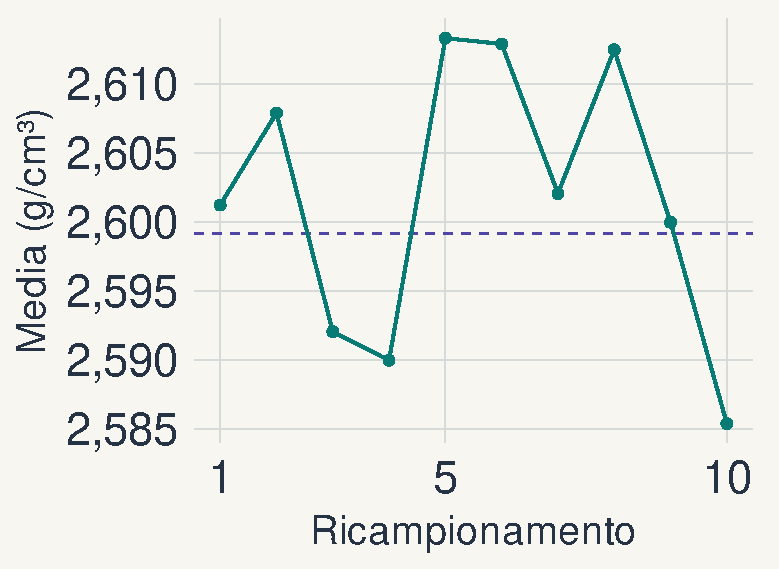
\includegraphics[width=\linewidth,height=6.15cm,keepaspectratio]{Figure/F02.pdf}\par}
\PSmall{Dieci medie ottenute dalle uniformi archiviate. Il controllo tra linguaggi usa le stesse righe nello stesso ordine.}
}};
\node[anchor=north west,inner sep=0] at([xshift=10.85cm,yshift=-2.12cm]current page.north west){\Colonna{8.16cm}{\PBody{Le dieci medie derivano dal medesimo piano casuale e vengono conservate come tabella di confronto fra implementazioni. La linea tratteggiata indica la media dei ventiquattro provini, rispetto alla quale le repliche oscillano perché cambiano le molteplicità delle osservazioni selezionate. Dieci ripetizioni sono sufficienti per questo controllo di corrispondenza e restano inadeguate per una stima accurata dei quantili di coda. Un uso inferenziale richiederebbe inoltre di valutare se ricampionare provini o stazioni rispetto alla domanda scientifica.}
}};
\end{tikzpicture}\end{frame}

\begin{frame}[plain]\hypertarget{slide39}{}
\bookmark[level=1,page=39]{Documentare l’ambiente e ricostruirlo}
\begin{tikzpicture}[remember picture,overlay]
\PilotChrome{Documentare l’ambiente e ricostruirlo}{CASUALITÀ E AMBIENTE DI ESECUZIONE}{39}{La documentazione dell’ambiente deve accompagnare una prova di esecuzione da condizioni iniziali dichiarate.}
\node[anchor=north west,inner sep=0] at([xshift=.96cm,yshift=-2.12cm]current page.north west){\Colonna{9.40cm}{\PLabel{Metodo}
\PBody{sessionInfo registra versione di R, piattaforma e pacchetti caricati, fornendo il contesto nel quale il risultato è stato ottenuto. La ricostruzione dell’ambiente richiede anche la disponibilità delle dipendenze e delle librerie di sistema, che possono variare fra piattaforme. Un elenco di versioni costituisce una testimonianza dell’esecuzione; un file di dipendenze risolte o un ambiente isolato ne facilita il ripristino. Il collaudo deve infine partire da una sessione pulita, affinché oggetti creati in precedenza non sostituiscano dipendenze mancanti.}
}};
\node[anchor=north west,inner sep=0] at([xshift=10.85cm,yshift=-2.12cm]current page.north west){\Colonna{8.16cm}{\PLabel{Interpretazione}
\PBody{La consegna conserva codice, dati utilizzati, versioni rilevate e registri di esecuzione. I risultati numerici vengono confrontati con tolleranze appropriate. Differenze di dispositivo grafico o libreria dei caratteri possono modificare la resa visiva pur lasciando invariati i valori sottostanti.}
}};
\end{tikzpicture}\end{frame}

\begin{frame}[plain]\hypertarget{slide40}{}
\bookmark[level=1,page=40]{Ripetere il seme ricostruisce il percorso casuale}
\begin{tikzpicture}[remember picture,overlay]
\PilotChrome{Ripetere il seme ricostruisce il percorso casuale}{CASUALITÀ E AMBIENTE DI ESECUZIONE}{40}{Le due sequenze ottenute ripristinando lo stato iniziale coincidono.}
\node[anchor=north west,inner sep=0] at([xshift=.96cm,yshift=-2.12cm]current page.north west){\Colonna{9.40cm}{\PLabel{Risultati del calcolo in R}
{\fontsize{10.2}{12.8}\selectfont\begin{tabular}{@{}>{\raggedright\arraybackslash}p{0.44\linewidth}@{\hspace{.13cm}}>{\raggedright\arraybackslash}p{0.48\linewidth}@{}}\toprule a & b\\[2.3pt]
\midrule 
0,15505 & 0,15505\\[2.3pt]
0,96838 & 0,96838\\[2.3pt]
0,40789 & 0,40789\\[2.3pt]
0,20689 & 0,20689\\[2.3pt]
0,1871 & 0,1871\\[2.3pt]
\bottomrule\end{tabular}\par}
\PSmall{Selezione di cinque righe dal file completo.}
}};
\node[anchor=north west,inner sep=0] at([xshift=10.85cm,yshift=-2.12cm]current page.north west){\Colonna{8.16cm}{\PBody{Quale confronto identifica una ripetizione nello stesso ambiente R?}
\vspace{.4cm}\PInfo{Le due sequenze ottenute ripristinando lo stato iniziale coincidono. L’aggiunta di una chiamata casuale intermedia cambia le estrazioni successive.}
}};
\node[anchor=north east,inner sep=0] at([xshift=17.1cm,yshift=-12.04cm]current page.north west){\fontsize{7.7}{9}\selectfont \href{https://github.com/marzione00/Lab_Geo/blob/649f7cc577b96bd1044d81e78a2f530813e4f96b/materiali/laboratori/M15/M15_N07.R}{\color{Classical}\bfseries Script R · M15\_N07}};
\end{tikzpicture}\end{frame}

\begin{frame}[plain]\hypertarget{slide41}{}
\bookmark[level=1,page=41]{Un piano comune permette di confrontare le repliche}
\begin{tikzpicture}[remember picture,overlay]
\PilotChrome{Un piano comune permette di confrontare le repliche}{CASUALITÀ E AMBIENTE DI ESECUZIONE}{41}{Gli indici del piano fissano quali densità entrano in ogni replica.}
\node[anchor=north west,inner sep=0] at([xshift=.96cm,yshift=-2.12cm]current page.north west){\Colonna{9.40cm}{\PLabel{Risultati del calcolo in R}
{\fontsize{10.2}{12.8}\selectfont\begin{tabular}{@{}>{\raggedright\arraybackslash}p{0.44\linewidth}@{\hspace{.13cm}}>{\raggedright\arraybackslash}p{0.48\linewidth}@{}}\toprule replica & media\\[2.3pt]
\midrule 
1 & 2,6012\\[2.3pt]
2 & 2,6079\\[2.3pt]
6 & 2,6129\\[2.3pt]
9 & 2,6\\[2.3pt]
10 & 2,5854\\[2.3pt]
\bottomrule\end{tabular}\par}
\PSmall{Selezione di cinque righe dal file completo.}
}};
\node[anchor=north west,inner sep=0] at([xshift=10.85cm,yshift=-2.12cm]current page.north west){\Colonna{8.16cm}{\PBody{Come riconoscere se due implementazioni hanno usato gli stessi campioni bootstrap?}
\vspace{.4cm}\PInfo{Gli indici del piano fissano quali densità entrano in ogni replica. Così un’eventuale differenza numerica si può ricondurre al calcolo sui dati selezionati.}
}};
\node[anchor=north east,inner sep=0] at([xshift=17.1cm,yshift=-12.04cm]current page.north west){\fontsize{7.7}{9}\selectfont \href{https://github.com/marzione00/Lab_Geo/blob/649f7cc577b96bd1044d81e78a2f530813e4f96b/materiali/laboratori/M15/M15_N08.R}{\color{Classical}\bfseries Script R · M15\_N08}};
\end{tikzpicture}\end{frame}

\begin{frame}[plain]\hypertarget{slide42}{}
\bookmark[level=1,page=42]{Seme casuale e stato del generatore}
\begin{tikzpicture}[remember picture,overlay]
\PilotChrome{Seme casuale e stato del generatore}{CASUALITÀ E AMBIENTE DI ESECUZIONE}{42}{Riprodurre una sequenza dichiarando il piano casuale.}
\node[anchor=north west,inner sep=0] at([xshift=.96cm,yshift=-2.12cm]current page.north west){\Colonna{9.40cm}{{\centering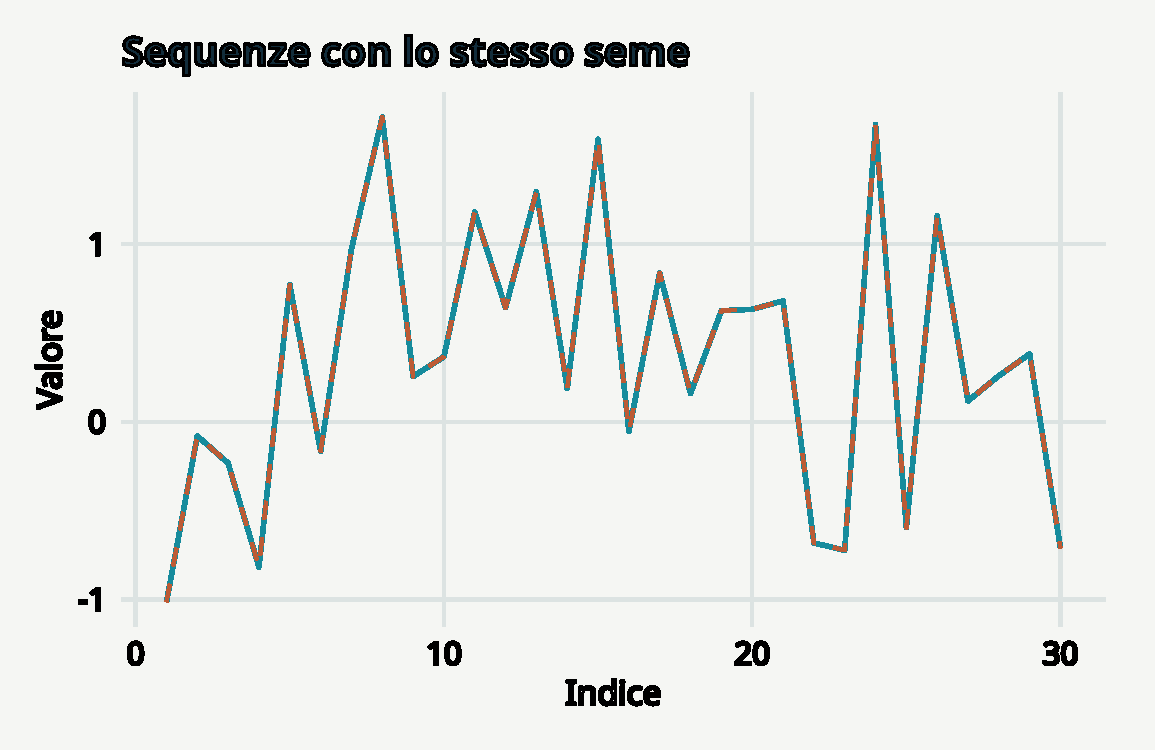
\includegraphics[width=\linewidth,height=6.0cm,keepaspectratio]{Esperimenti/m15-casualita-A.pdf}\par}
\PSmall{Estrazioni preliminari: 0. Seme: 17.}
}};
\node[anchor=north west,inner sep=0] at([xshift=10.85cm,yshift=-2.12cm]current page.north west){\Colonna{8.16cm}{\PLabel{Scenario A · simulazione}
\PBody{Un generatore pseudocasuale produce una sequenza determinata dal proprio stato e dall’ordine delle chiamate. Il programma inizializza due volte il generatore con lo stesso seme; nella seconda esecuzione può consumare alcune estrazioni preliminari prima di registrare i valori confrontati. Le due curve mostrano come questo cambiamento sposti la sequenza osservata.}
\par\smallskip{\centering\adjustbox{max width=.98\linewidth}{$\displaystyle X=G(s,\text{ordine delle chiamate})$}\par\smallskip}
\PSmall{G indica il generatore pseudocasuale, s il suo stato iniziale determinato dal seme e X la sequenza restituita. L’ordine delle chiamate include anche estrazioni che non vengono successivamente utilizzate nel risultato.}
}};
\node[anchor=north east,inner sep=0] at([xshift=17.1cm,yshift=-12.04cm]current page.north west){\fontsize{7.7}{9}\selectfont \href{https://marzione00.github.io/Lab_Geo/\#laboratorio/m15-casualita}{\color{Classical}\bfseries Apri il laboratorio · m15-casualita}};
\end{tikzpicture}\end{frame}

\begin{frame}[plain]\hypertarget{slide43}{}
\bookmark[level=1,page=43]{Confronto | Seme casuale e stato del generatore}
\begin{tikzpicture}[remember picture,overlay]
\PilotChrome{Confronto | Seme casuale e stato del generatore}{CASUALITÀ E AMBIENTE DI ESECUZIONE}{43}{Il seme iniziale, l’algoritmo e l’ordine delle chiamate concorrono alla sequenza riproducibile.}
\node[anchor=north west,inner sep=0] at([xshift=.96cm,yshift=-2.12cm]current page.north west){\Colonna{9.40cm}{{\centering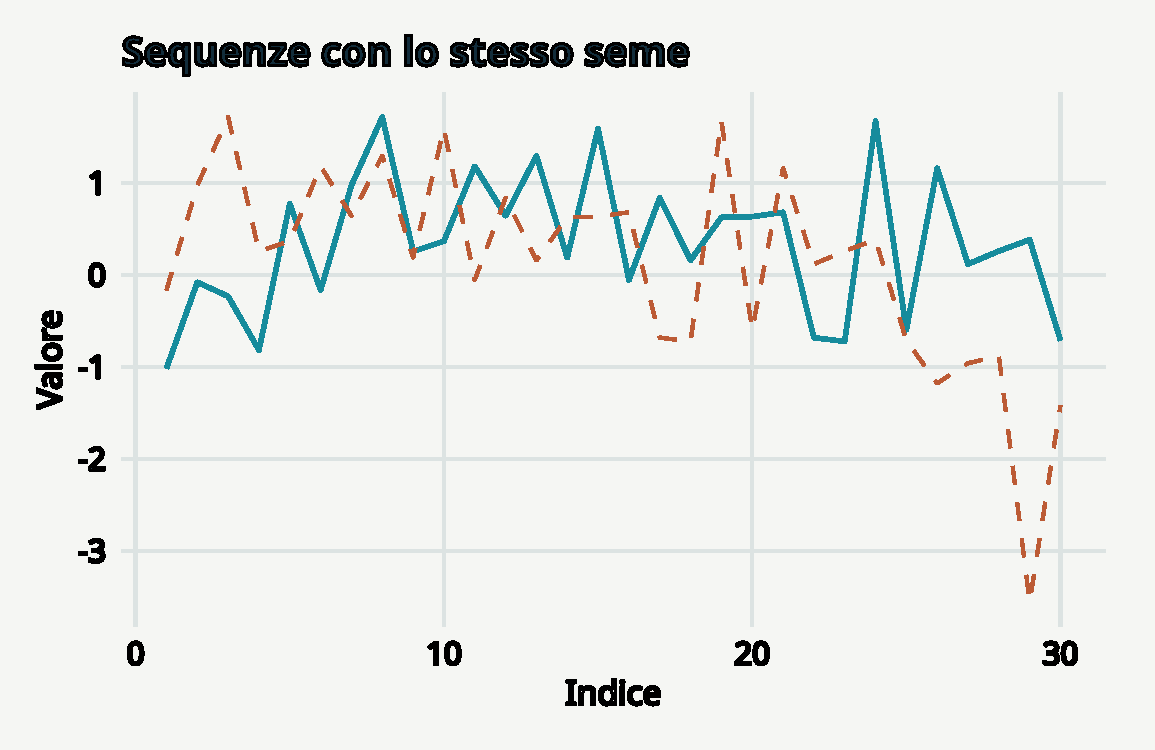
\includegraphics[width=\linewidth,height=5.6cm,keepaspectratio]{Esperimenti/m15-casualita-B.pdf}\par}
\PSmall{Estrazioni preliminari: 0 $\to$ 5. Tutti gli altri parametri e il seme sono fissi.}
}};
\node[anchor=north west,inner sep=0] at([xshift=10.85cm,yshift=-2.12cm]current page.north west){\Colonna{8.16cm}{\PLabel{Confronto fra gli scenari}
{\fontsize{10.2}{12.8}\selectfont\begin{tabular}{@{}>{\raggedright\arraybackslash}p{0.48\linewidth}@{\hspace{.13cm}}>{\raggedright\arraybackslash}p{0.224\linewidth}@{\hspace{.13cm}}>{\raggedright\arraybackslash}p{0.224\linewidth}@{}}\toprule Grandezza & A & B\\[2.3pt]
\midrule 
Sequenze identiche & sì & no\\[2.3pt]
Scarto massimo & 0 & 3,94\\[2.3pt]
Estrazioni preliminari & 0 & 5\\[2.3pt]
\bottomrule\end{tabular}\par}
\vspace{.25cm}\PBody{Cinque estrazioni preliminari spostano lo stato del generatore. Anche con lo stesso seme iniziale le sequenze usate nell’analisi divergono.}
}};
\node[anchor=north east,inner sep=0] at([xshift=17.1cm,yshift=-12.04cm]current page.north west){\fontsize{7.7}{9}\selectfont \href{https://marzione00.github.io/Lab_Geo/\#laboratorio/m15-casualita}{\color{Classical}\bfseries Apri il laboratorio · m15-casualita}};
\end{tikzpicture}\end{frame}

\begin{frame}[plain]\hypertarget{slide44}{}
\bookmark[level=0,page=44]{Parametri, versioni e provenienza}
\bookmark[level=1,page=44]{La soglia seleziona anche la popolazione descritta}
\begin{tikzpicture}[remember picture,overlay]
\PilotChrome{La soglia seleziona anche la popolazione descritta}{PARAMETRI, VERSIONI E PROVENIENZA}{44}{Conserva valore della soglia, numero di righe ed elenco degli identificativi coinvolti.}
\node[anchor=north west,inner sep=0] at([xshift=.96cm,yshift=-2.12cm]current page.north west){\Colonna{9.40cm}{\PLabel{Domanda}
\PBody{Tre campioni hanno volumi di 40, 45 e 50 cm³. Se l’analisi richiede almeno 45 cm³, quale campione scompare?}
\vspace{.35cm}\PLabel{Interpretazione}
\PBody{L’identificativo escluso va registrato. Cambia il sottoinsieme a cui attribuiamo la sintesi e il risultato può cambiare anche con la stessa funzione di calcolo.}
}};
\node[anchor=north west,inner sep=0] at([xshift=10.85cm,yshift=-2.12cm]current page.north west){\Colonna{8.16cm}{\begin{tcolorbox}[enhanced,arc=1.7mm,boxrule=.6pt,colback=white,colframe=Classical!60!Navy,colbacktitle=Navy,coltitle=white,fonttitle=\bfseries\small,title={R · calcolo riproducibile},left=1.7mm,right=1.3mm,top=1.1mm,bottom=1.1mm,before skip=1mm,after skip=1.0mm]\lstinputlisting[style=GeoR,language=R]{Codice/capitolo-05.R}\end{tcolorbox}
\PLabel{Risultato in R}
\begin{tcolorbox}[colback=GeoTint,colframe=Rule,boxrule=.5pt,arc=1.4mm,left=2mm,right=1mm,top=1mm,bottom=1mm]{\fontsize{9}{12}\selectfont\ttfamily \mbox{prima\ \ dopo\ }\\\mbox{\ \ \ \ 3\ \ \ \ \ 2\ }\\\mbox{[1]\ "C01"}}\end{tcolorbox}}};
\end{tikzpicture}\end{frame}

\begin{frame}[plain]\hypertarget{slide45}{}
\bookmark[level=1,page=45]{Una soglia modifica il campione analizzato}
\begin{tikzpicture}[remember picture,overlay]
\PilotChrome{Una soglia modifica il campione analizzato}{PARAMETRI, VERSIONI E PROVENIENZA}{45}{Una proprietà matematica del filtro aiuta a verificare l’implementazione, mentre la soglia richiede una motivazione.}
\node[anchor=north west,inner sep=0] at([xshift=.96cm,yshift=-2.12cm]current page.north west){\Colonna{9.40cm}{{\centering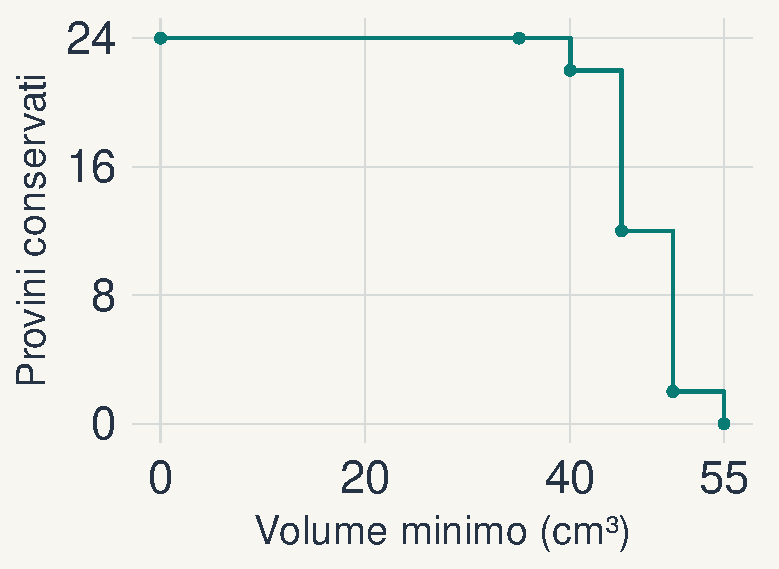
\includegraphics[width=\linewidth,height=6.15cm,keepaspectratio]{Figure/F04.pdf}\par}
\PSmall{$V_i$: volume del provino i; c: soglia in cm³; A(c): identificativi conservati. Il grafico mostra la loro numerosità.}
}};
\node[anchor=north west,inner sep=0] at([xshift=10.85cm,yshift=-2.12cm]current page.north west){\Colonna{8.16cm}{\PBody{La soglia sul volume viene registrata in un file di parametri e applicata con una disuguaglianza esplicita. Aumentandola, il numero dei provini conservati può soltanto diminuire o restare invariato, poiché gli insiemi selezionati sono annidati. Questa proprietà fornisce un controllo del codice. Il valore della soglia richiede invece una motivazione legata al protocollo di misura, alla qualità del provino o alla domanda di ricerca; la sua visibilità nel file rende la decisione ispezionabile senza giustificarla automaticamente.}
\par\smallskip{\centering\adjustbox{max width=.98\linewidth}{$\displaystyle A(c)=\{i:V_i\geq c\},\qquad c_2>c_1\Rightarrow A(c_2)\subseteq A(c_1)$}\par\smallskip}
}};
\end{tikzpicture}\end{frame}

\begin{frame}[plain]\hypertarget{slide46}{}
\bookmark[level=1,page=46]{Sensibilità della sintesi al criterio di selezione}
\begin{tikzpicture}[remember picture,overlay]
\PilotChrome{Sensibilità della sintesi al criterio di selezione}{PARAMETRI, VERSIONI E PROVENIENZA}{46}{La sensibilità di una sintesi deve essere letta insieme alla composizione del campione che la sostiene.}
\node[anchor=north west,inner sep=0] at([xshift=.96cm,yshift=-2.12cm]current page.north west){\Colonna{9.40cm}{{\centering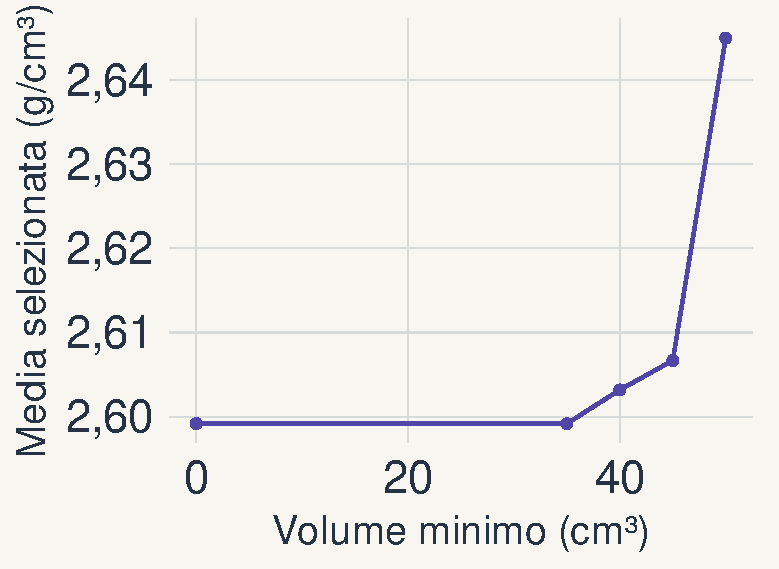
\includegraphics[width=\linewidth,height=6.15cm,keepaspectratio]{Figure/F05.pdf}\par}
\PSmall{Media delle densità dopo ciascun filtro sul volume. A 55 cm³ nessun provino resta disponibile e la media è indefinita.}
}};
\node[anchor=north west,inner sep=0] at([xshift=10.85cm,yshift=-2.12cm]current page.north west){\Colonna{8.16cm}{\PBody{La media delle densità cambia quando il filtro elimina provini con caratteristiche diverse da quelle conservate. La curva permette di esaminare tale dipendenza per soglie di volume minimo pari a 0, 35, 40, 45, 50 e 55 cm³. Un tratto stabile riguarda soltanto i valori e i criteri considerati, mentre un cambiamento marcato suggerisce di esaminare quali stazioni e quali provini siano stati esclusi. Il confronto va accompagnato dai conteggi, poiché una media calcolata su pochi campioni può apparire simile alla media complessiva pur avendo un supporto osservativo molto diverso.}
}};
\end{tikzpicture}\end{frame}

\begin{frame}[plain]\hypertarget{slide47}{}
\bookmark[level=1,page=47]{Registrare la decisione e le osservazioni coinvolte}
\begin{tikzpicture}[remember picture,overlay]
\PilotChrome{Registrare la decisione e le osservazioni coinvolte}{PARAMETRI, VERSIONI E PROVENIENZA}{47}{Il registro rende ricostruibile il rapporto fra scelta analitica e risultato.}
\node[anchor=north west,inner sep=0] at([xshift=.96cm,yshift=-2.12cm]current page.north west){\Colonna{9.40cm}{{\centering\resizebox{.97\linewidth}{!}{\begin{tikzpicture}[x=1cm,y=-.87cm,every node/.style={font=\fontsize{12.2}{15}\selectfont,text=Ink},arr/.style={-{Stealth[length=2mm]},line width=.8pt,draw=Classical}]\path[use as bounding box] (0,0) rectangle (7.45,6.2);
\draw[draw=Classical,fill=Classical!8,rounded corners=2pt,line width=.7pt] (0.5,0.4) rectangle (6.9,1.5499999999999998);
\node[anchor=center,text=Ink,font=\fontsize{11.5}{15}\selectfont,text width=6cm,align=center] at (3.7,0.975) {Regola, unità e motivazione};
\draw[arr,draw=Classical] (3.7,1.7000000000000002)--(3.7,2.08);
\draw[draw=Quantum,fill=Quantum!8,rounded corners=2pt,line width=.7pt] (0.5,2.25) rectangle (6.9,3.4);
\node[anchor=center,text=Ink,font=\fontsize{11.5}{15}\selectfont,text width=6cm,align=center] at (3.7,2.825) {Identificativi e conteggi prima/dopo};
\draw[arr,draw=Classical] (3.7,3.55)--(3.7,3.9299999999999997);
\draw[draw=Classical,fill=Classical!8,rounded corners=2pt,line width=.7pt] (0.5,4.1000000000000005) rectangle (6.9,5.25);
\node[anchor=center,text=Ink,font=\fontsize{11.5}{15}\selectfont,text width=6cm,align=center] at (3.7,4.675000000000001) {Effetto sulla conclusione};

\end{tikzpicture}}\par}
}};
\node[anchor=north west,inner sep=0] at([xshift=10.85cm,yshift=-2.12cm]current page.north west){\Colonna{8.16cm}{\PBody{Il registro delle decisioni associa a ogni trasformazione una regola, una motivazione, il momento della scelta e gli identificativi interessati. I conteggi prima e dopo il filtro permettono di controllare l’effetto complessivo, mentre l’elenco dei provini esclusi consente di verificare eventuali concentrazioni per stazione. La data di esecuzione documenta l’elaborazione e deve rimanere distinta dalla data di campionamento. Se una soglia viene modificata dopo aver osservato i risultati, anche questa circostanza entra nella descrizione del procedimento.}
}};
\end{tikzpicture}\end{frame}

\begin{frame}[plain]\hypertarget{slide48}{}
\bookmark[level=1,page=48]{Commit e differenze nel codice}
\begin{tikzpicture}[remember picture,overlay]
\PilotChrome{Commit e differenze nel codice}{PARAMETRI, VERSIONI E PROVENIENZA}{48}{La storia delle modifiche acquista valore quando è collegata alle ragioni e alle conseguenze delle decisioni.}
\node[anchor=north west,inner sep=0] at([xshift=.96cm,yshift=-2.12cm]current page.north west){\Colonna{9.40cm}{{\centering\resizebox{.97\linewidth}{!}{\begin{tikzpicture}[x=1cm,y=-.87cm,every node/.style={font=\fontsize{12.2}{15}\selectfont,text=Ink},arr/.style={-{Stealth[length=2mm]},line width=.8pt,draw=Classical}]\path[use as bounding box] (0,0) rectangle (7.45,6.2);
\draw[draw=Classical,fill=Classical!8,rounded corners=2pt,line width=.7pt] (0.5,0.8) rectangle (3.2,2.8);
\node[anchor=center,text=Ink,font=\fontsize{12.2}{15}\selectfont,text width=2.4cm,align=center] at (1.85,1.8) {Versione A\par soglia = 4};
\draw[draw=Quantum,fill=Quantum!8,rounded corners=2pt,line width=.7pt] (4.2,0.8) rectangle (6.9,2.8);
\node[anchor=center,text=Ink,font=\fontsize{12.2}{15}\selectfont,text width=2.4cm,align=center] at (5.55,1.8) {Versione B\par soglia = 5};
\draw[arr,draw=Classical] (3.4,1.8)--(4,1.8);
\node[anchor=center,text=Ink,font=\fontsize{12.2}{15}\selectfont,text width=6cm,align=center] at (3.7,4) {Diff: modifica osservabile};
\node[anchor=center,text=Ink,font=\fontsize{11.5}{15}\selectfont,text width=6.6cm,align=center] at (3.7,5.3) {Commit: stato e motivazione del cambiamento};

\end{tikzpicture}}\par}
}};
\node[anchor=north west,inner sep=0] at([xshift=10.85cm,yshift=-2.12cm]current page.north west){\Colonna{8.16cm}{\PBody{Un sistema di versionamento conserva stati riconoscibili dei file e permette di confrontare le modifiche. Prima di registrare un commit si esamina il diff, collegando le righe cambiate alla motivazione scientifica e agli effetti attesi. Il laboratorio crea un repository locale e modifica una soglia dimostrativa, senza richiedere un servizio remoto. La cronologia del codice permette di ricostruire il cambiamento, mentre il messaggio e il registro delle decisioni ne esplicitano il significato per l’analisi.}
}};
\end{tikzpicture}\end{frame}

\begin{frame}[plain]\hypertarget{slide49}{}
\bookmark[level=1,page=49]{File locali e regole di esclusione}
\begin{tikzpicture}[remember picture,overlay]
\PilotChrome{File locali e regole di esclusione}{PARAMETRI, VERSIONI E PROVENIENZA}{49}{Le regole di esclusione devono essere verificate rispetto ai file effettivamente tracciati e distribuiti.}
\node[anchor=north west,inner sep=0] at([xshift=.96cm,yshift=-2.12cm]current page.north west){\Colonna{9.40cm}{\PLabel{Metodo}
\PBody{La regola gitignore controlla l’inclusione ordinaria dei file ancora non tracciati, consentendo di separare prodotti rigenerabili, configurazioni locali e sorgenti condivisi. Un file già registrato mantiene la propria storia anche quando viene aggiunto a una regola di esclusione. Nel laboratorio si utilizza un segnaposto privo di credenziali reali per osservare il comportamento del comando check-ignore. Il contenuto effettivamente incluso in una consegna deve essere verificato nell’archivio finale, poiché le regole del repository e la selezione dei file distribuiti possono differire.}
}};
\node[anchor=north west,inner sep=0] at([xshift=10.85cm,yshift=-2.12cm]current page.north west){\Colonna{8.16cm}{\PLabel{Interpretazione}
\PBody{Le figure definitive possono essere distribuite insieme al codice che le produce, mentre file temporanei e risultati intermedi rigenerabili possono essere esclusi. La scelta dipende dalla funzione del pacchetto: esecuzione, revisione scientifica oppure consultazione didattica.}
}};
\end{tikzpicture}\end{frame}

\begin{frame}[plain]\hypertarget{slide50}{}
\bookmark[level=1,page=50]{Risposte di servizi e copie locali verificabili}
\begin{tikzpicture}[remember picture,overlay]
\PilotChrome{Risposte di servizi e copie locali verificabili}{PARAMETRI, VERSIONI E PROVENIENZA}{50}{La provenienza di una risposta deve essere conservata prima della sua trasformazione in tabella.}
\node[anchor=north west,inner sep=0] at([xshift=.96cm,yshift=-2.12cm]current page.north west){\Colonna{9.40cm}{{\centering\resizebox{.97\linewidth}{!}{\begin{tikzpicture}[x=1cm,y=-.87cm,every node/.style={font=\fontsize{12.2}{15}\selectfont,text=Ink},arr/.style={-{Stealth[length=2mm]},line width=.8pt,draw=Classical}]\path[use as bounding box] (0,0) rectangle (7.45,6.2);
\draw[draw=Classical,fill=Classical!8,rounded corners=2pt,line width=.7pt] (0.5,0.4) rectangle (6.9,1.5499999999999998);
\node[anchor=center,text=Ink,font=\fontsize{11.5}{15}\selectfont,text width=6cm,align=center] at (3.7,0.975) {Richiesta e metadati di accesso};
\draw[arr,draw=Classical] (3.7,1.7000000000000002)--(3.7,2.08);
\draw[draw=Quantum,fill=Quantum!8,rounded corners=2pt,line width=.7pt] (0.5,2.25) rectangle (6.9,3.4);
\node[anchor=center,text=Ink,font=\fontsize{11.5}{15}\selectfont,text width=6cm,align=center] at (3.7,2.825) {Risposta grezza conservata};
\draw[arr,draw=Classical] (3.7,3.55)--(3.7,3.9299999999999997);
\draw[draw=Classical,fill=Classical!8,rounded corners=2pt,line width=.7pt] (0.5,4.1000000000000005) rectangle (6.9,5.25);
\node[anchor=center,text=Ink,font=\fontsize{11.5}{15}\selectfont,text width=6cm,align=center] at (3.7,4.675000000000001) {Schema verificato e tabella derivata};

\end{tikzpicture}}\par}
}};
\node[anchor=north west,inner sep=0] at([xshift=10.85cm,yshift=-2.12cm]current page.north west){\Colonna{8.16cm}{\PBody{Una risposta acquisita da un servizio può cambiare quando variano dati, parametri o versione dell’interfaccia. Conservare la risposta grezza insieme a indirizzo, parametri pubblici, data di accesso, unità e condizioni d’uso rende possibile una successiva verifica. Il laboratorio usa un JSON costruito localmente, nel quale due osservazioni hanno identificativi e valori in metri. La natura dimostrativa del file rimane esplicita: il controllo dello schema esercita la lettura di una risposta senza attribuirle una provenienza osservativa reale.}
}};
\end{tikzpicture}\end{frame}

\begin{frame}[plain]\hypertarget{slide51}{}
\bookmark[level=1,page=51]{Manifest e consegna riproducibile}
\begin{tikzpicture}[remember picture,overlay]
\PilotChrome{Manifest e consegna riproducibile}{PARAMETRI, VERSIONI E PROVENIENZA}{51}{La consegna deve consentire sia l’esecuzione sia l’esame critico delle scelte scientifiche.}
\node[anchor=north west,inner sep=0] at([xshift=.96cm,yshift=-2.12cm]current page.north west){\Colonna{9.40cm}{\PLabel{Metodo}
\PBody{Il manifest elenca i file distribuiti con dimensione e impronta, permettendo di riconoscere assenze e modifiche rispetto alla versione consegnata. Il lettore deve inoltre disporre di istruzioni per avviare gli script, informazioni sull’ambiente e una descrizione dei risultati attesi. I laboratori N01–N06 sviluppano struttura e integrità; N07–N12 casualità e prove; N13–N19 parametri, versioni e provenienza; N20 riunisce i passaggi nella sintesi per stazione. L’esercizio conclusivo richiede una nuova esecuzione da una sessione pulita e il confronto dei risultati.}
}};
\node[anchor=north west,inner sep=0] at([xshift=10.85cm,yshift=-2.12cm]current page.north west){\Colonna{8.16cm}{\PLabel{Interpretazione}
\PBody{La relazione finale distingue l’identità dei file, l’equivalenza numerica dei risultati e la validità scientifica della procedura. Per ciascun livello indica il controllo eseguito, il riferimento utilizzato e le condizioni entro le quali il confronto è pertinente.}
}};
\end{tikzpicture}\end{frame}

\begin{frame}[plain]\hypertarget{slide52}{}
\bookmark[level=1,page=52]{Un filtro esplicito può lasciare intatto il campione}
\begin{tikzpicture}[remember picture,overlay]
\PilotChrome{Un filtro esplicito può lasciare intatto il campione}{PARAMETRI, VERSIONI E PROVENIENZA}{52}{Nel caso mostrato la soglia mantiene tutte le 24 righe.}
\node[anchor=north west,inner sep=0] at([xshift=.96cm,yshift=-2.12cm]current page.north west){\Colonna{9.40cm}{\PLabel{Risultati del calcolo in R}
{\fontsize{10.2}{12.8}\selectfont\begin{tabular}{@{}>{\raggedright\arraybackslash}p{0.52\linewidth}@{\hspace{.13cm}}>{\raggedright\arraybackslash}p{0.39\linewidth}@{}}\toprule Grandezza & Valore\\[2.3pt]
\midrule 
Soglia & 4\\[2.3pt]
n prima & 24\\[2.3pt]
n dopo & 24\\[2.3pt]
\bottomrule\end{tabular}\par}
}};
\node[anchor=north west,inner sep=0] at([xshift=10.85cm,yshift=-2.12cm]current page.north west){\Colonna{8.16cm}{\PBody{Il parametro corrente elimina davvero qualche osservazione?}
\vspace{.4cm}\PInfo{Nel caso mostrato la soglia mantiene tutte le 24 righe. Registrare la soglia resta necessario anche quando il risultato corrente coincide con quello iniziale.}
}};
\node[anchor=north east,inner sep=0] at([xshift=17.1cm,yshift=-12.04cm]current page.north west){\fontsize{7.7}{9}\selectfont \href{https://github.com/marzione00/Lab_Geo/blob/649f7cc577b96bd1044d81e78a2f530813e4f96b/materiali/laboratori/M15/M15_N13.R}{\color{Classical}\bfseries Script R · M15\_N13}};
\end{tikzpicture}\end{frame}

\begin{frame}[plain]\hypertarget{slide53}{}
\bookmark[level=1,page=53]{Il registro descrive la decisione analitica}
\begin{tikzpicture}[remember picture,overlay]
\PilotChrome{Il registro descrive la decisione analitica}{PARAMETRI, VERSIONI E PROVENIENZA}{53}{Un registro con conteggi e motivazione permette di rivedere la scelta.}
\node[anchor=north west,inner sep=0] at([xshift=.96cm,yshift=-2.12cm]current page.north west){\Colonna{9.40cm}{\PLabel{Risultati del calcolo in R}
{\fontsize{10.2}{12.8}\selectfont\begin{tabular}{@{}>{\raggedright\arraybackslash}p{0.52\linewidth}@{\hspace{.13cm}}>{\raggedright\arraybackslash}p{0.39\linewidth}@{}}\toprule Grandezza & Valore\\[2.3pt]
\midrule 
passaggio & volume positivo\\[2.3pt]
n prima & 24\\[2.3pt]
n dopo & 24\\[2.3pt]
motivazione & vincolo fisico\\[2.3pt]
\bottomrule\end{tabular}\par}
}};
\node[anchor=north west,inner sep=0] at([xshift=10.85cm,yshift=-2.12cm]current page.north west){\Colonna{8.16cm}{\PBody{Che cosa deve sapere chi tenta di applicare di nuovo lo stesso filtro?}
\vspace{.4cm}\PInfo{Un registro con conteggi e motivazione permette di rivedere la scelta. Gli identificativi esclusi diventano essenziali appena una riga viene eliminata.}
}};
\node[anchor=north east,inner sep=0] at([xshift=17.1cm,yshift=-12.04cm]current page.north west){\fontsize{7.7}{9}\selectfont \href{https://github.com/marzione00/Lab_Geo/blob/649f7cc577b96bd1044d81e78a2f530813e4f96b/materiali/laboratori/M15/M15_N14.R}{\color{Classical}\bfseries Script R · M15\_N14}};
\end{tikzpicture}\end{frame}

\begin{frame}[plain]\hypertarget{slide54}{}
\bookmark[level=1,page=54]{La sintesi finale torna alle stazioni}
\begin{tikzpicture}[remember picture,overlay]
\PilotChrome{La sintesi finale torna alle stazioni}{PARAMETRI, VERSIONI E PROVENIENZA}{54}{La media è calcolata all’interno di ogni stazione.}
\node[anchor=north west,inner sep=0] at([xshift=.96cm,yshift=-2.12cm]current page.north west){\Colonna{9.40cm}{\PLabel{Risultati del calcolo in R}
{\fontsize{10.2}{12.8}\selectfont\begin{tabular}{@{}>{\raggedright\arraybackslash}p{0.44\linewidth}@{\hspace{.13cm}}>{\raggedright\arraybackslash}p{0.48\linewidth}@{}}\toprule stazione & dens\\[2.3pt]
\midrule 
A1 & 2,685\\[2.3pt]
A2 & 2,6525\\[2.3pt]
B1 & 2,5925\\[2.3pt]
B2 & 2,5475\\[2.3pt]
B3 & 2,5125\\[2.3pt]
\bottomrule\end{tabular}\par}
\PSmall{Selezione di cinque righe dal file completo.}
}};
\node[anchor=north west,inner sep=0] at([xshift=10.85cm,yshift=-2.12cm]current page.north west){\Colonna{8.16cm}{\PBody{Quale risultato deve ricomparire rigenerando la tabella dalla sorgente?}
\vspace{.4cm}\PInfo{La media è calcolata all’interno di ogni stazione. L’identificativo e l’unità della densità devono accompagnare il valore esportato.}
}};
\node[anchor=north east,inner sep=0] at([xshift=17.1cm,yshift=-12.04cm]current page.north west){\fontsize{7.7}{9}\selectfont \href{https://github.com/marzione00/Lab_Geo/blob/649f7cc577b96bd1044d81e78a2f530813e4f96b/materiali/laboratori/M15/M15_N20.R}{\color{Classical}\bfseries Script R · M15\_N20}};
\end{tikzpicture}\end{frame}

\begin{frame}[plain]\hypertarget{slide55}{}
\bookmark[level=1,page=55]{Parametri, versioni e sensibilità}
\begin{tikzpicture}[remember picture,overlay]
\PilotChrome{Parametri, versioni e sensibilità}{PARAMETRI, VERSIONI E PROVENIENZA}{55}{Confrontare risultati prodotti da scelte analitiche tracciate.}
\node[anchor=north west,inner sep=0] at([xshift=.96cm,yshift=-2.12cm]current page.north west){\Colonna{9.40cm}{{\centering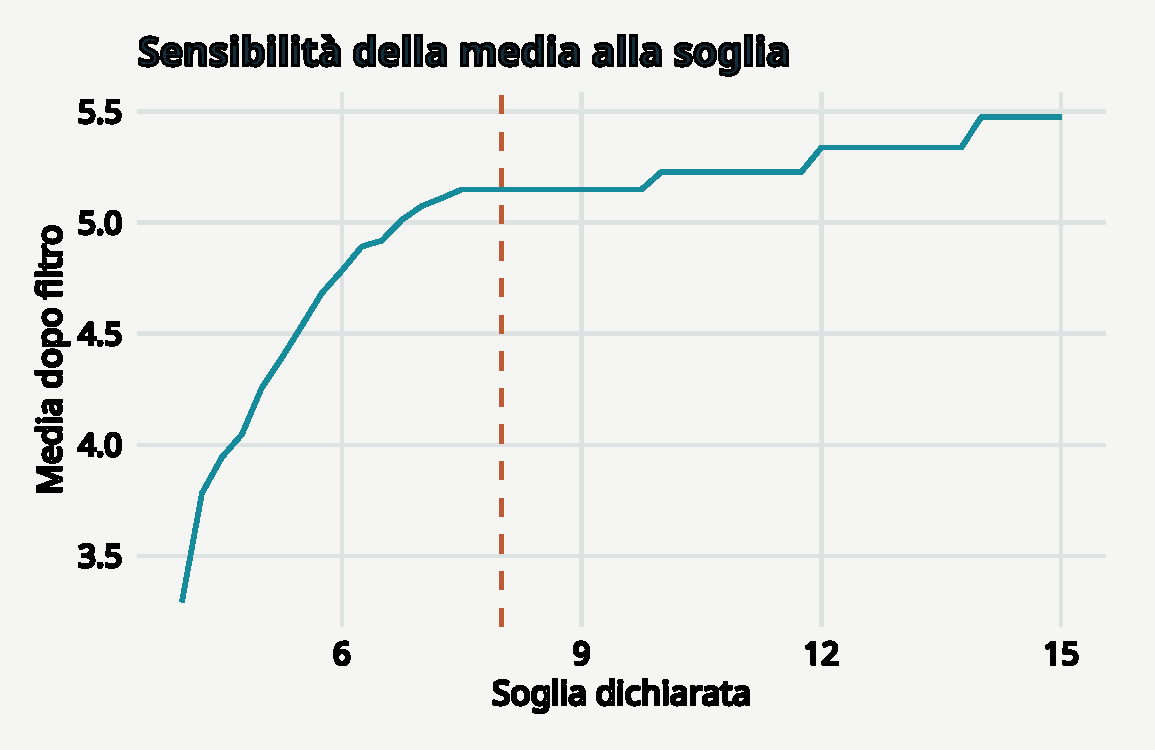
\includegraphics[width=\linewidth,height=6.0cm,keepaspectratio]{Esperimenti/m15-provenienza-A.pdf}\par}
\PSmall{Soglia superiore della versione corrente: 8. Seme: 17.}
}};
\node[anchor=north west,inner sep=0] at([xshift=10.85cm,yshift=-2.12cm]current page.north west){\Colonna{8.16cm}{\PLabel{Scenario A · simulazione}
\PBody{Una soglia di filtro modifica quali osservazioni contribuiscano alla sintesi di un campione. L’esperimento combina misure gaussiane sintetiche con alcuni valori elevati e calcola la media dopo diverse soglie superiori. Il controllo individua la configurazione corrente, della quale vengono riportati il risultato e il numero di osservazioni ammesse.}
\par\smallskip{\centering\adjustbox{max width=.98\linewidth}{$\displaystyle \widehat\theta=f(D;\eta,\mathcal V)$}\par\smallskip}
\PSmall{$\hat{\theta}$ è la sintesi prodotta dalla funzione f; D sono i dati, η i parametri dell’analisi e V l’ambiente o la versione del procedimento. Nell’esperimento il parametro modificabile è la soglia superiore di inclusione.}
}};
\node[anchor=north east,inner sep=0] at([xshift=17.1cm,yshift=-12.04cm]current page.north west){\fontsize{7.7}{9}\selectfont \href{https://marzione00.github.io/Lab_Geo/\#laboratorio/m15-provenienza}{\color{Classical}\bfseries Apri il laboratorio · m15-provenienza}};
\end{tikzpicture}\end{frame}

\begin{frame}[plain]\hypertarget{slide56}{}
\bookmark[level=1,page=56]{Confronto | Parametri, versioni e sensibilità}
\begin{tikzpicture}[remember picture,overlay]
\PilotChrome{Confronto | Parametri, versioni e sensibilità}{PARAMETRI, VERSIONI E PROVENIENZA}{56}{Una configurazione esportata conserva parametri, dati e codice necessari alla ricostruzione.}
\node[anchor=north west,inner sep=0] at([xshift=.96cm,yshift=-2.12cm]current page.north west){\Colonna{9.40cm}{{\centering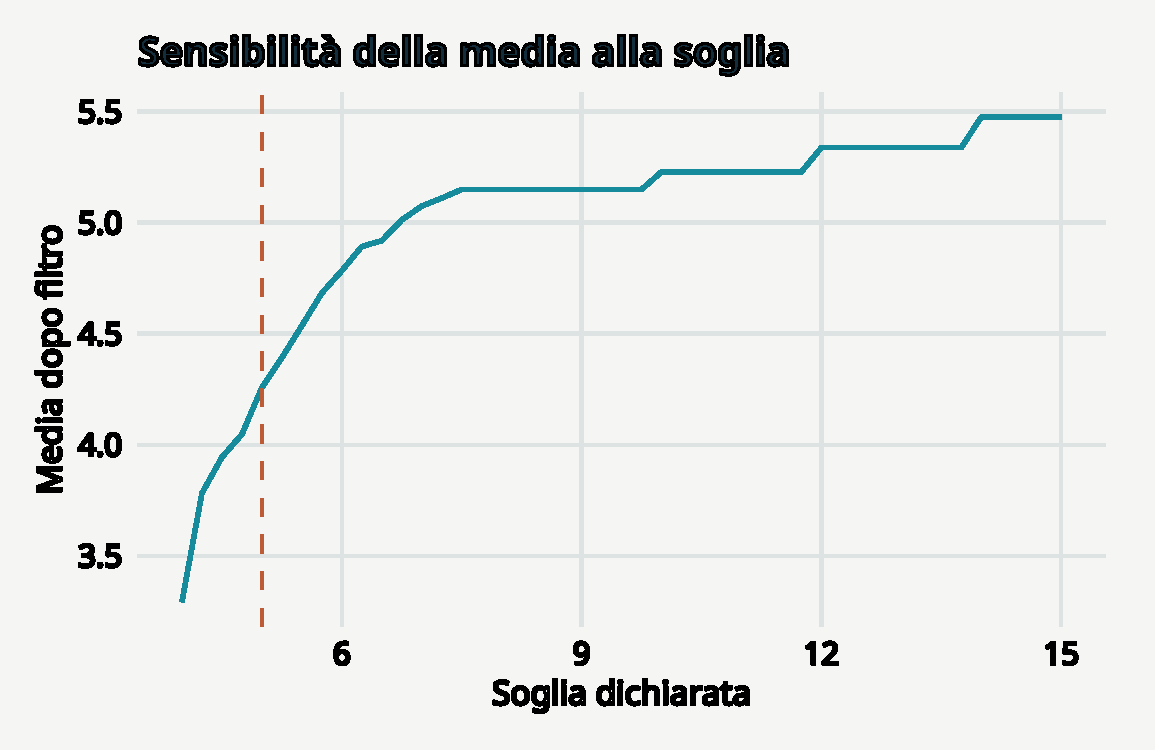
\includegraphics[width=\linewidth,height=5.6cm,keepaspectratio]{Esperimenti/m15-provenienza-B.pdf}\par}
\PSmall{Soglia superiore della versione corrente: 8 $\to$ 5. Tutti gli altri parametri e il seme sono fissi.}
}};
\node[anchor=north west,inner sep=0] at([xshift=10.85cm,yshift=-2.12cm]current page.north west){\Colonna{8.16cm}{\PLabel{Confronto fra gli scenari}
{\fontsize{10.2}{12.8}\selectfont\begin{tabular}{@{}>{\raggedright\arraybackslash}p{0.48\linewidth}@{\hspace{.13cm}}>{\raggedright\arraybackslash}p{0.224\linewidth}@{\hspace{.13cm}}>{\raggedright\arraybackslash}p{0.224\linewidth}@{}}\toprule Grandezza & A & B\\[2.3pt]
\midrule 
Soglia corrente & 8 & 5\\[2.3pt]
Media corrente & 5,15 & 4,26\\[2.3pt]
Osservazioni incluse & 60 & 27\\[2.3pt]
\bottomrule\end{tabular}\par}
\vspace{.25cm}\PBody{Con la soglia più restrittiva il sottoinsieme passa da 60 a 27 osservazioni. La differenza fra le medie va letta insieme alla modifica del campione.}
}};
\node[anchor=north east,inner sep=0] at([xshift=17.1cm,yshift=-12.04cm]current page.north west){\fontsize{7.7}{9}\selectfont \href{https://marzione00.github.io/Lab_Geo/\#laboratorio/m15-provenienza}{\color{Classical}\bfseries Apri il laboratorio · m15-provenienza}};
\end{tikzpicture}\end{frame}

\begin{frame}[plain]\hypertarget{slide57}{}
\bookmark[level=1,page=57]{Dal risultato alla relazione}
\begin{tikzpicture}[remember picture,overlay]
\PilotChrome{Dal risultato alla relazione}{SINTESI}{57}{Consegna dati, dizionario, codice, parametri, ambiente e confronto numerico con un riferimento.}
\node[anchor=north west,inner sep=0] at([xshift=.96cm,yshift=-2.12cm]current page.north west){\Colonna{9.40cm}{\PLabel{Domanda di partenza}
\PBody{Quali informazioni permettono di ricostruire la media delle densità di una stazione?}
\PLabel{Risultato da discutere}
\PBody{La media di A1 è 2,685 g/cm³ sui quattro provini del dataset. Un’altra persona può ricostruirla dividendo masse per volumi e aggregando per lo stesso ID di stazione.}
}};
\node[anchor=north west,inner sep=0] at([xshift=10.85cm,yshift=-2.12cm]current page.north west){\Colonna{8.16cm}{\PLabel{Limiti della conclusione}
\PBody{Una sintesi ripetibile può comunque dipendere da misure distorte o da una selezione inadeguata. Verificare il procedimento e interpretare il campione sono compiti complementari.}
\vspace{.4cm}\href{https://marzione00.github.io/Lab_Geo/\#modulo-P10}{\color{Classical}\bfseries Prosegui · P10 · Un’analisi ricostruibile e verificabile}}};
\end{tikzpicture}\end{frame}

\begin{frame}[plain]\hypertarget{slide58}{}
\bookmark[level=1,page=58]{Fonti, dati e codice per riprodurre le figure}
\begin{tikzpicture}[remember picture,overlay]
\PilotChrome{Fonti, dati e codice per riprodurre le figure}{RIFERIMENTI}{58}{Ogni valore pubblicato deve poter essere ricollegato ai dati di ingresso.}
\node[anchor=north west,inner sep=0] at([xshift=.96cm,yshift=-2.12cm]current page.north west){\Colonna{9.40cm}{\PLabel{Materiali del corso}
\PBody{Il fascicolo deriva dal modulo M15 di GeoStat Lab e dai materiali didattici di Marzio De Corato. I dati del caso guida sono didattici. Le simulazioni A e B riportano il proprio seme.}
\href{https://github.com/marzione00/Lab_Geo/blob/649f7cc577b96bd1044d81e78a2f530813e4f96b/moduli/M15/README.md}{\color{Classical}\bfseries Scheda e documentazione originale}\par\smallskip \href{https://github.com/marzione00/Lab_Geo/blob/649f7cc577b96bd1044d81e78a2f530813e4f96b/materiali/R/M15_figure.R}{\color{Classical}\bfseries Script R delle figure del corso}}};
\node[anchor=north west,inner sep=0] at([xshift=10.85cm,yshift=-2.12cm]current page.north west){\Colonna{8.16cm}{\PLabel{Nell’archivio dei sorgenti}
\PBody{Codice contiene i frammenti delle pagine. Esperimenti comprende i due programmi R e i risultati di ciascun confronto. Diagrammi contiene i disegni TikZ modificabili. Scena conserva il modello Blender della copertina.}
\vspace{.4cm}\href{https://marzione00.github.io/Lab_Geo/\#modulo-M15}{\color{Classical}\bfseries Apri Argenta su GeoStat Lab}}};
\end{tikzpicture}\end{frame}

\end{document}